\documentclass[a4paper]{article}

\usepackage[pdftex,
  hidelinks,
  pdfauthor={Dexter Chua},
  pdfsubject={Cambridge Maths Notes: Part IB - Electromagnetism},
  pdftitle={Part IB - Electromagnetism},
pdfkeywords={Cambridge Mathematics Maths Math IB Lent Electromagnetism}]{hyperref}

\title{Part IB - Electromagnetism}
\author{Lectured by David Tong}
\date{Lent 2015}

% Imports
\ifx \nextra \undefined
  \usepackage[pdftex,
    hidelinks,
    pdfauthor={Dexter Chua},
    pdfsubject={Cambridge Maths Notes: Part \npart\ - \ncourse},
    pdftitle={Part \npart\ - \ncourse},
  pdfkeywords={Cambridge Mathematics Maths Math \npart\ \nterm\ \nyear\ \ncourse}]{hyperref}
  \title{Part \npart\ - \ncourse}
\else
  \usepackage[pdftex,
    hidelinks,
    pdfauthor={Dexter Chua},
    pdfsubject={Cambridge Maths Notes: Part \npart\ - \ncourse\ (\nextra)},
    pdftitle={Part \npart\ - \ncourse\ (\nextra)},
  pdfkeywords={Cambridge Mathematics Maths Math \npart\ \nterm\ \nyear\ \ncourse\ \nextra}]{hyperref}

  \title{Part \npart\ - \ncourse \\ {\Large \nextra}}
\fi

\author{Lectured by \nlecturer \\\small Notes taken by Dexter Chua}
\date{\nterm\ \nyear}

\usepackage{alltt}
\usepackage{amsfonts}
\usepackage{amsmath}
\usepackage{amssymb}
\usepackage{amsthm}
\usepackage{booktabs}
\usepackage{caption}
\usepackage{enumitem}
\usepackage{fancyhdr}
\usepackage{graphicx}
\usepackage{mathtools}
\usepackage{microtype}
\usepackage{multirow}
\usepackage{pdflscape}
\usepackage{pgfplots}
\usepackage{siunitx}
\usepackage{tabularx}
\usepackage{tikz}
\usepackage{tkz-euclide}
\usepackage[normalem]{ulem}
\usepackage[all]{xy}

\pgfplotsset{compat=1.12}

\pagestyle{fancyplain}
\lhead{\emph{\nouppercase{\leftmark}}}
\ifx \nextra \undefined
  \rhead{
    \ifnum\thepage=1
    \else
      \npart\ \ncourse
    \fi}
\else
  \rhead{
    \ifnum\thepage=1
    \else
      \npart\ \ncourse\ (\nextra)
    \fi}
\fi
\usetikzlibrary{arrows}
\usetikzlibrary{decorations.markings}
\usetikzlibrary{decorations.pathmorphing}
\usetikzlibrary{positioning}
\usetikzlibrary{fadings}
\usetikzlibrary{intersections}
\usetikzlibrary{cd}

\newcommand*{\Cdot}{\raisebox{-0.25ex}{\scalebox{1.5}{$\cdot$}}}
\newcommand {\pd}[2][ ]{
  \ifx #1 { }
    \frac{\partial}{\partial #2}
  \else
    \frac{\partial^{#1}}{\partial #2^{#1}}
  \fi
}

% Theorems
\theoremstyle{definition}
\newtheorem*{aim}{Aim}
\newtheorem*{axiom}{Axiom}
\newtheorem*{claim}{Claim}
\newtheorem*{cor}{Corollary}
\newtheorem*{defi}{Definition}
\newtheorem*{eg}{Example}
\newtheorem*{fact}{Fact}
\newtheorem*{law}{Law}
\newtheorem*{lemma}{Lemma}
\newtheorem*{notation}{Notation}
\newtheorem*{prop}{Proposition}
\newtheorem*{thm}{Theorem}

\renewcommand{\labelitemi}{--}
\renewcommand{\labelitemii}{$\circ$}
\renewcommand{\labelenumi}{(\roman{*})}

\let\stdsection\section
\renewcommand\section{\newpage\stdsection}

% Strike through
\def\st{\bgroup \ULdepth=-.55ex \ULset}

% Maths symbols
\newcommand{\bra}{\langle}
\newcommand{\ket}{\rangle}

\newcommand{\N}{\mathbb{N}}
\newcommand{\Z}{\mathbb{Z}}
\newcommand{\Q}{\mathbb{Q}}
\renewcommand{\H}{\mathbb{H}}
\newcommand{\R}{\mathbb{R}}
\newcommand{\C}{\mathbb{C}}
\newcommand{\Prob}{\mathbb{P}}
\renewcommand{\P}{\mathbb{P}}
\newcommand{\E}{\mathbb{E}}
\newcommand{\F}{\mathbb{F}}
\newcommand{\cU}{\mathcal{U}}
\newcommand{\RP}{\mathbb{RP}}
\newcommand{\CP}{\mathbb{CP}}

\newcommand{\ph}{\,\cdot\,}

\DeclareMathOperator{\sech}{sech}
\DeclareMathOperator{\cosech}{cosech}
\DeclareMathOperator{\cosec}{cosec}

\DeclareMathOperator{\covol}{covol}
\DeclareMathOperator{\vol}{vol}

\let\Im\relax
\let\Re\relax
\DeclareMathOperator{\Im}{Im}
\DeclareMathOperator{\Re}{Re}
\DeclareMathOperator{\im}{im}
\DeclareMathOperator{\image}{image}
\DeclareMathOperator{\Ann}{Ann}

\DeclareMathOperator*{\res}{res}
\DeclareMathOperator{\Res}{Res}
\DeclareMathOperator{\Ind}{Ind}

\DeclareMathOperator{\tr}{tr}
\DeclareMathOperator{\diag}{diag}
\DeclareMathOperator{\rank}{rank}
\DeclareMathOperator{\card}{card}
\DeclareMathOperator{\spn}{span}
\DeclareMathOperator{\adj}{adj}

\DeclareMathOperator{\erf}{erf}
\DeclareMathOperator{\erfc}{erfc}

\DeclareMathOperator{\ord}{ord}
\DeclareMathOperator{\Sym}{Sym}

\DeclareMathOperator{\sgn}{sgn}
\DeclareMathOperator{\orb}{orb}
\DeclareMathOperator{\stab}{stab}
\DeclareMathOperator{\ccl}{ccl}

\DeclareMathOperator{\lcm}{lcm}
\DeclareMathOperator{\hcf}{hcf}

\DeclareMathOperator{\Int}{Int}
\DeclareMathOperator{\id}{id}

\DeclareMathOperator{\betaD}{beta}
\DeclareMathOperator{\gammaD}{gamma}
\DeclareMathOperator{\Poisson}{Poisson}
\DeclareMathOperator{\binomial}{binomial}
\DeclareMathOperator{\multinomial}{multinomial}
\DeclareMathOperator{\Bernoulli}{Bernoulli}
\DeclareMathOperator{\like}{like}

\DeclareMathOperator{\var}{var}
\DeclareMathOperator{\cov}{cov}
\DeclareMathOperator{\bias}{bias}
\DeclareMathOperator{\mse}{mse}
\DeclareMathOperator{\corr}{corr}

\DeclareMathOperator{\otp}{otp}
\DeclareMathOperator{\dom}{dom}

\DeclareMathOperator{\Root}{Root}
\DeclareMathOperator{\supp}{supp}
\DeclareMathOperator{\rel}{rel}
\DeclareMathOperator{\Hom}{Hom}
\DeclareMathOperator{\Aut}{Aut}
\DeclareMathOperator{\Gal}{Gal}
\DeclareMathOperator{\Mat}{Mat}
\DeclareMathOperator{\End}{End}
\DeclareMathOperator{\Char}{char}
\DeclareMathOperator{\ev}{ev}
\DeclareMathOperator{\St}{St}
\DeclareMathOperator{\Lk}{Lk}
\DeclareMathOperator{\disc}{disc}
\DeclareMathOperator{\Isom}{Isom}
\DeclareMathOperator{\length}{length}
\DeclareMathOperator{\energy}{energy}
\DeclareMathOperator{\area}{area}
\DeclareMathOperator{\Syl}{Syl}
\DeclareMathOperator{\cl}{cl}
\DeclareMathOperator{\fix}{fix}

\newcommand{\GL}{\mathrm{GL}}
\newcommand{\SL}{\mathrm{SL}}
\newcommand{\PGL}{\mathrm{PGL}}
\newcommand{\PSL}{\mathrm{PSL}}
\newcommand{\PSU}{\mathrm{PSU}}
\newcommand{\Or}{\mathrm{O}}
\newcommand{\SO}{\mathrm{SO}}
\newcommand{\U}{\mathrm{U}}
\newcommand{\SU}{\mathrm{SU}}

\renewcommand{\d}{\mathrm{d}}
\newcommand{\D}{\mathrm{D}}

\tikzset{->/.style = {decoration={markings,
                                  mark=at position 1 with {\arrow[scale=2]{latex'}}},
                      postaction={decorate}}}
\tikzset{<-/.style = {decoration={markings,
                                  mark=at position 0 with {\arrowreversed[scale=2]{latex'}}},
                      postaction={decorate}}}
\tikzset{<->/.style = {decoration={markings,
                                   mark=at position 0 with {\arrowreversed[scale=2]{latex'}},
                                   mark=at position 1 with {\arrow[scale=2]{latex'}}},
                       postaction={decorate}}}
\tikzset{->-/.style = {decoration={markings,
                                   mark=at position #1 with {\arrow[scale=2]{latex'}}},
                       postaction={decorate}}}
\tikzset{-<-/.style = {decoration={markings,
                                   mark=at position #1 with {\arrowreversed[scale=2]{latex'}}},
                       postaction={decorate}}}

\tikzset{circ/.style = {fill, circle, inner sep = 0, minimum size = 3}}
\tikzset{mstate/.style={circle, draw, blue, text=black, minimum width=0.7cm}}

\definecolor{mblue}{rgb}{0.2, 0.3, 0.8}
\definecolor{morange}{rgb}{1, 0.5, 0}
\definecolor{mgreen}{rgb}{0.1, 0.4, 0.2}
\definecolor{mred}{rgb}{0.5, 0, 0}

\def\drawcirculararc(#1,#2)(#3,#4)(#5,#6){%
    \pgfmathsetmacro\cA{(#1*#1+#2*#2-#3*#3-#4*#4)/2}%
    \pgfmathsetmacro\cB{(#1*#1+#2*#2-#5*#5-#6*#6)/2}%
    \pgfmathsetmacro\cy{(\cB*(#1-#3)-\cA*(#1-#5))/%
                        ((#2-#6)*(#1-#3)-(#2-#4)*(#1-#5))}%
    \pgfmathsetmacro\cx{(\cA-\cy*(#2-#4))/(#1-#3)}%
    \pgfmathsetmacro\cr{sqrt((#1-\cx)*(#1-\cx)+(#2-\cy)*(#2-\cy))}%
    \pgfmathsetmacro\cA{atan2(#2-\cy,#1-\cx)}%
    \pgfmathsetmacro\cB{atan2(#6-\cy,#5-\cx)}%
    \pgfmathparse{\cB<\cA}%
    \ifnum\pgfmathresult=1
        \pgfmathsetmacro\cB{\cB+360}%
    \fi
    \draw (#1,#2) arc (\cA:\cB:\cr);%
}
\newcommand\getCoord[3]{\newdimen{#1}\newdimen{#2}\pgfextractx{#1}{\pgfpointanchor{#3}{center}}\pgfextracty{#2}{\pgfpointanchor{#3}{center}}}

\def\Xint#1{\mathchoice
   {\XXint\displaystyle\textstyle{#1}}%
   {\XXint\textstyle\scriptstyle{#1}}%
   {\XXint\scriptstyle\scriptscriptstyle{#1}}%
   {\XXint\scriptscriptstyle\scriptscriptstyle{#1}}%
   \!\int}
\def\XXint#1#2#3{{\setbox0=\hbox{$#1{#2#3}{\int}$}
     \vcenter{\hbox{$#2#3$}}\kern-.5\wd0}}
\def\ddashint{\Xint=}
\def\dashint{\Xint-}


\begin{document}
\maketitle
{\small
\noindent\textbf{Electromagnetism and Relativity}\\
Review of Special Relativity; tensors and index notation. Lorentz force law. Electromagnetic tensor. Lorentz transformations of electric and magnetic fields. Currents and the conservation of charge. Maxwell equations in relativistic and non-relativistic forms.\hspace*{\fill} [5]

\vspace{10pt}
\noindent\textbf{Electrostatics}\\
Gauss's law. Application to spherically symmetric and cylindrically symmetric charge distributions.  Point, line and surface charges. Electrostatic potentials; general charge distributions, dipoles. Electrostatic energy. Conductors.\hspace*{\fill} [3]

\vspace{10pt}
\noindent\textbf{Magnetostatics}\\
Magnetic fields due to steady currents. Ampre's law. Simple examples. Vector potentials and the Biot-Savart law for general current distributions. Magnetic dipoles. Lorentz force on current distributions and force between current-carrying wires. Ohm's law.\hspace*{\fill} [3]

\vspace{10pt}
\noindent\textbf{Electrodynamics}\\
Faraday's law of induction for fixed and moving circuits. Electromagnetic energy and Poynting vector.  4-vector potential, gauge transformations. Plane electromagnetic waves in vacuum, polarization.\hspace*{\fill} [5]}

\tableofcontents
\section{Introduction}
Electromagnetism is important.
\subsection{Charge and Current}
The strength of the electromagnetic force experienced by a particle is determined by its \emph{(electric) charge}. The SI unit of charge is the \emph{Coulomb}. In this course, we assume that the charge can be any real number. However, at the fundamental level, charge is quantised. All particles carry charge $q = ne$ with $n\in \Z$, \footnote{Actually quarks have $n = \pm1/3$ or $\pm2/3$, but when we study quarks, electromagnetism becomes insignificant compared to the strong force. So for all practical purposes we can have $n\in \Z$.} and the basic unit $e \approx 1.6 \times 10^{-19} $C. For example, the electron has $n = -1$, proton has $n = +1$, neutron = $n = 0$.

In this course, it will be more useful to talk about \emph{charge density} $\rho(\mathbf{x}, t)$.
\begin{defi}[Charge density]
  The \emph{charge density} is the charge per unit volume. The total charge in a region $V$ is
  \[
    Q = \int_V \rho(\mathbf{x}, t)\; \d V
  \]
\end{defi}

The motion of charge is described by the \emph{current} density $\mathbf{J}(\mathbf{x}, t)$.
\begin{defi}[Current and current density]
For any surface $S$, the integral
\[
  I = \int_S \mathbf{J}\cdot d\mathbf{S}
\]
counts the charge per unit time passing through $S$. $I$ is the \emph{current}, and $\mathbf{J}$ is the \emph{charge density}, ``current per unit area''.
\end{defi}
Intuitively, if the charge distribution $\rho (\mathbf{x}, t)$ has velocity $\mathbf{v}(x, t)$, then (neglecting relativistic effects), we have
\[
  \mathbf{J} = \rho \mathbf{v}
\]

\begin{eg}
  A wire is a cylinder of cross-sectional area $A$. Suppose there are $n$ electrons per unit volume. Then
  \begin{align*}
    \rho &= nq = -ne\\
    \mathbf{J} &= nq\mathbf{v}\\
    I &= nqvA
  \end{align*}
\end{eg}

It is well know that charge is conserved. However, we can have a stronger statement- charge is conserved locally: it is not possible that a charge in a box disappears and instantaneously appears on the moon. If it disappears in the box, it must have moved to somewhere nearby.

This is captured by the \emph{continuity equation}.
\begin{law}[Continuity equation]
  \[
    \frac{\partial\rho}{\partial t} + \nabla\cdot \mathbf{J} = 0
  \]
\end{law}
The charge $Q$ in some region $V$ is
\[
  Q = \int_V \rho \;\d V
\]
So
\[
  \frac{\d Q}{\d t} = \int_V \frac{\partial\rho}{\partial t}\; \d V = -\int_V \nabla\cdot \mathbf{J}\; \d V = -\int_S \mathbf{J}\cdot \d S
\]
where the last equality is by the divergence theorem. ie. the rate of change in charge is the rate of charge flowing out of the point.

We can take $V = \R^3$, the whole of space. If there are no currents at infinity, then
\[
  \frac{\d Q}{\d t} = 0
\]
So the continuity equation implies the conservation of charge.

\subsection{Forces and Fields}
All forces are mediated by \emph{fields}. In physics a \emph{field} is a dynamical quantity which takes values at every point in space and time. The electromagnetic force is mediated by two fields:
\begin{itemize}
  \item electric field $\mathbf{E}(\mathbf{x}, t)$
  \item magnetic field $\mathbf{B}(\mathbf{x}, t)$
\end{itemize}
Each of these fields is itself a 3-vector. There are two aspects to the force:
\begin{itemize}
  \item Particles create fields
  \item Fields move particles
\end{itemize}
The second aspect is governed by the Lorentz force law:
\begin{law}[Lorentz force law]
\[
  \mathbf{F} = q(\mathbf{E} + \mathbf{v}\times \mathbf{B})
\]
\end{law}
The first aspect is governed by \emph{Maxwell's equations}.
\begin{law}[Maxwell's Equations]
  \begin{align*}
    \nabla \cdot \mathbf{E} &= \frac{\rho}{\varepsilon_0}\\
    \nabla \cdot \mathbf{B} &= 0\\
    \nabla \times \mathbf{E} +\frac{\partial \mathbf{B}}{\partial t} &= 0\\
    \nabla \times \mathbf{B} - \mu_0\varepsilon_0 \frac{\partial \mathbf{E}}{\partial t} &= \mu_0 \mathbf{j}
  \end{align*}
  where
  \begin{itemize}
    \item $\varepsilon_0 = \SI{8.85e-12}{\per\metre\cubed\per\kilogram\s\squared\coulomb\squared}$ is the electric constant
    \item $\mu_0 = \SI{4\pi e-6}{\metre\kilogram\per\coulomb\squared}$ is the magnetic constant
  \end{itemize}
\end{law}
These equations are special in a mathematical way. In fact, using quantum mechanics and relativity, it can be shown that these are the only equations that can possibly describe electromagnetism.

\section{Electrostatics}
Take a stationary charge density $\rho = \rho(\mathbf{x})$ with $\mathbf{J} = 0$. We look for time-independent solutions with $\mathbf{B} = 0$. We are left with two equations
\begin{align*}
  \nabla \cdot \mathbf{E} &= \frac{\rho}{\varepsilon_0}\\
  \nabla\times \mathbf{E} &= 0
\end{align*}
and the other two equations just give $0 = 0$. Our goal is: Given $\rho$, find $\mathbf{E}$.
\subsection{Gauss' Law}
Consider a region $V\subseteq \R^3$ with boundary $S = \partial V$. We integrate the first equation over $V$:
\[
  \int \nabla\cdot \mathbf{E}\; \d V = \int_S \mathbf{E}\cdot \d \mathbf{S} = \frac{1}{\varepsilon_0} \int_V \rho \;\d V.
\]
So
\begin{law}[Gauss' law]
  \[
    \int_S \mathbf{E}\cdot \d \mathbf{S} =\frac{Q}{\varepsilon_0},
  \]
  where $Q$ is the total charge inside $V$.
\end{law}
\begin{defi}[Flux through surface]
  The \emph{flux} of $\mathbf{E}$ through the surface $S$ is defined to be 
  \[
    \int_S \mathbf{E} \cdot\d \mathbf{S}.
  \]
\end{defi}

\note All surfaces containing charge $Q$ have the same flux. Only charge inside $S$ contributes to the flux. If there is a charge outside, then the field lines go in through one side of the surface and leave through the other. Then it gives no total flux.

From this, we can prove Coulomb's law:
\begin{eg}
  Gauss' law $\Rightarrow$ Coulomb's force law.

  We consider a spherically symmetric charge density $\rho (r)$. with $\rho (r) = 0$ for $r > R$, ie. all the charge is contained in a ball of radius $R$.

  \begin{center}
    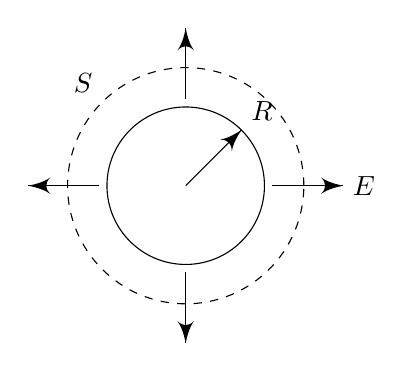
\begin{tikzpicture}
      \draw circle [radius=1];
      \draw [->] (0, 0) -- (.71, .71) node [anchor=south west] {$R$};
      \draw [->] (0, 1.1) -- (0, 2);
      \draw [->] (0, -1.1) -- (0, -2);
      \draw [->] (1.1, 0) -- (2, 0) node [right] {$E$};
      \draw [->] (-1.1, 0) -- (-2, 0);
      \draw [dashed] circle [radius=1.5];
      \node at (-1.06, 1.06) [anchor=south east] {$S$};
    \end{tikzpicture}
  \end{center}

  By symmetry, the force is the same in all directions and point outward radially. So
  \[
    \mathbf{E} = E(r) \hat{\mathbf{r}}.
  \]
  This immediately ensures that $\nabla \times \mathbf{E} = 0$.

  Put $S$ to be a sphere of radius $r > R$. Then
  \begin{align*}
    \int_S \mathbf{E}\cdot \d \mathbf{S} &= \int_S E(r) \hat{\mathbf{r}}\cdot \d \mathbf{S}\\
    &= E(r) \int_S \hat{\mathbf{r}}\cdot \d \mathbf{S}\\
    &= E(r)\cdot 4\pi r^2\\
    &= \frac{Q}{\varepsilon_0}
  \end{align*}
  We were able to pull the $E(r)$ out since it is constant over the sphere.

  Therefore
  \[
    \mathbf{E}(r) = \frac{Q}{4\pi\varepsilon_0 r^2}\hat{\mathbf{r}}.
  \]
  The Lorentz force law tells us that the force experienced by a second charge is
  \[
    \mathbf{F}(\mathbf{r}) = \frac{Qq}{4\pi\varepsilon_0 r^2}\hat{\mathbf{r}},
  \]
  which is Coulomb's law. Note that strictly speaking, this only holds when the charges are not moving. However, we can still use this because the corrections when they move are tiny.
\end{eg}

\begin{eg}
  Consider a uniform sphere with
  \[
    \rho (r) = \begin{cases}
      \rho & r < R\\
      0 & r > R
    \end{cases}.
  \]
  Outside, we know that 
  \[
    \mathbf{E} = \frac{Q}{4\pi\varepsilon_0 r^2}\hat{\mathbf{r}}
  \]

  Now suppose we are inside the sphere.
   \begin{center}
    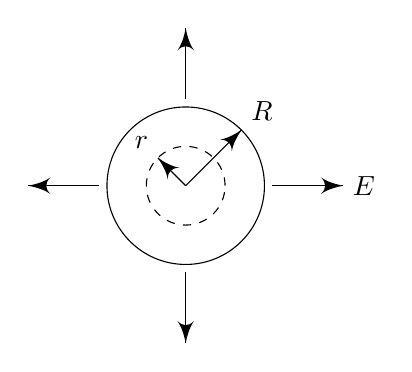
\begin{tikzpicture}
      \draw circle [radius=1];
      \draw [->] (0, 0) -- (.71, .71) node [anchor=south west] {$R$};
      \draw [->] (0, 1.1) -- (0, 2);
      \draw [->] (0, -1.1) -- (0, -2);
      \draw [->] (1.1, 0) -- (2, 0) node [right] {$E$};
      \draw [->] (-1.1, 0) -- (-2, 0);
      \draw [dashed] circle [radius=0.5];
      \draw [->] (0, 0) -- (-.353, .353) node [anchor=south east] {$r$};
    \end{tikzpicture}
  \end{center}

  Then
  \begin{align*}
    \int_S \mathbf{E}\cdot \d\mathbf{S} &= E(r) 4\pi r^2\\
    &= \frac{Q}{\varepsilon_0}\left(\frac{r^3}{R^3}\right)
  \end{align*}
  
  So 
  \[
    \mathbf{E}(r) = \frac{Qr}{4\pi\varepsilon_0 R^3}\hat{\mathbf{r}},
  \]
  and the field increases with radius. 
\end{eg}

\begin{eg}[Line charge]
  Consider an infinite line with uniform charge density \emph{per unit length} $\eta$.

  We use cylindrical polar coordinates:
  \begin{center}
    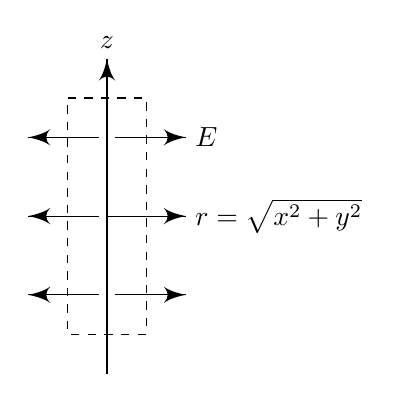
\begin{tikzpicture}
      \draw [->] (0, -2) -- (0, 2) node [above] {$z$};
      \draw [->] (0, 0) -- (1, 0) node [right] {$r = \sqrt{x^2 + y^2}$};

      \draw [->] (0.1, 1) -- (1, 1) node [right] {$E$};
      \draw [->] (-0.1, 1) -- (-1, 1);
      \draw [->] (-0.1, 0) -- (-1, 0);
      \draw [->] (0.1, -1) -- (1, -1);
      \draw [->] (-0.1, -1) -- (-1, -1);

      \draw [dashed] (-0.5, 1.5) -- (0.5, 1.5) -- (0.5, -1.5) -- (-0.5, -1.5) -- cycle;
    \end{tikzpicture}
  \end{center}

  By symmetry, the field is radial, ie.
  \[
    \mathbf{E}(r) = E(r) \hat{\mathbf{r}}.
  \]
  Pick $S$ to be a cylinder of length $L$ and radius $r$. We know that the end caps do not contribute to the flux since the field lines are perpendicular to the normal. Also, the curved surface has area $2\pi rL$. Then
  \[
    \int_S\mathbf{E}\cdot \d\mathbf{S} = E(r)2\pi rL = \frac{\eta L}{\varepsilon_0}.
  \]
  So
  \[
    \mathbf{E}(r) = \frac{\eta}{2\pi \varepsilon_0 r} \hat{\mathbf{r}}.
  \]
  Note that the field varies as $1/r$, not $1/r^2$. Intuitively, this is because we have one more dimension of ``stuff'' compared to the point charge, so the field does not drop as fast.
\end{eg}

\begin{eg}[Surface charge]
  Consider an infinite plane $z = 0$, with uniform charge per unit area $\sigma$.

  \begin{center}
    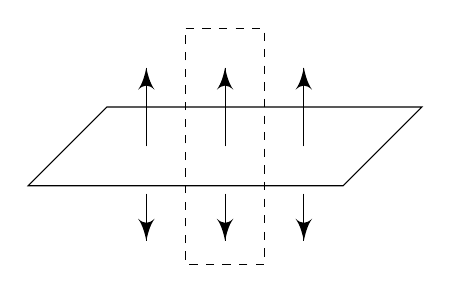
\begin{tikzpicture}
      \draw (-2.5, -.5) -- (1.5, -.5) -- (2.5, .5) -- (-1.5, .5) -- cycle;
      \draw [->] (0, 0) -- (0, 1);
      \draw [->] (-1, 0) -- (-1, 1);
      \draw [->] (1, 0) -- (1, 1);
      
      \draw [->] (0, -.6) -- (0, -1.2);
      \draw [->] (1, -.6) -- (1, -1.2);
      \draw [->] (-1, -.6) -- (-1, -1.2);

      \draw [dashed] (-0.5, 1.5) -- (0.5, 1.5) -- (0.5, -1.5) -- (-0.5, -1.5) -- cycle;
    \end{tikzpicture}
  \end{center}

  By symmetry, the field points vertically, and the field bottom is the opposite of that on top. we must have
  \[
    \mathbf{E} = E(z)\hat{\mathbf{z}}
  \]
  with
  \[
    E(z) = -E(-z).
  \]
  Consider a vertical cylinder of height $2z$ and cross-sectional area $A$. Now only the end caps contribute.
  \begin{align*}
    \int_S \mathbf{E} \cdot \d \mathbf{S} &= E(z) A - E(-z) A\\
    &=\frac{\sigma A}{\varepsilon _0}. 
  \end{align*}
  So
  \[
    E(z) = \frac{\sigma }{2\varepsilon_0}
  \]
  and is constant.

  Note that the electric field is discontinuous across the surface. We have
  \[
    E(z\to 0+) - E(z\to 0-) = \frac{\sigma}{\varepsilon_0}.
  \]
  Note that this is a general result that is true for any arbitrary surfaces and $\sigma$. We can prove this by considering a cylinder across the surface and then shrink it indefinitely. The we find that
  \[
    \hat{\mathbf{n}}\cdot \mathbf{E}_+ - \hat{\mathbf{n}}\cdot \mathbf{E}_- = \frac{\sigma}{\varepsilon_0}.
  \]
  However, the components of $\mathbf{E}$ tangential to the surface are continuous. 
\end{eg}

\subsection{Electrostatic potential}
In general, we will have to solve both $\nabla \cdot \mathbf{E} = \rho/\varepsilon_0$ and $\nabla \times \mathbf{E} = \mathbf{0}$. However, we already know that the general form of the solution to the second equation is $\mathbf{E} = -\nabla\phi$ for some scalar field $\phi$.
\begin{defi}[Electrostatic potential]
  If $\mathbf{E} = -\nabla \phi$, then $\phi$ is the \emph{electrostatic potential}.
\end{defi}
Then
\[
  \nabla\cdot \mathbf{E} = \frac{\rho}{\varepsilon_0} \Rightarrow \nabla^2\phi = \frac{\rho}{\varepsilon_0},
\]
which is the \emph{Poisson equation}. If we are in the middle of nowhere and $\rho = 0$, then we just get the \emph{Laplace equation}.

Note the following:
\begin{itemize}
  \item $\phi$ is only defined up to a constant. We usually fix this by insisting $\phi(\mathbf{r}) \to 0$ as $r\to \infty$. Note that this statement seems trivial, but this property of $\phi$ is actually very important and gives rise to a lot of interesting properties, as we will see later.
  \item The Poisson equation is linear. So if we have two charges $\rho = \rho_1 + \rho_1$, then $\phi = \phi_1 + \phi_2$ and $\mathbf{E} = \mathbf{E}_i + \mathbf{E}_2$. This is the \emph{principle of superposition}. Among the four fundamental forces of nature, electromagnetism is the only force with this property.
\end{itemize}
\subsubsection{Point charge}
Consider a point particle with charge $Q$ at the origin. Then
\[
  \rho (\mathbf{r}) = Q\delta^3(\mathbf{r}).
\]
The power 3 of the delta function indicates that it is for a 3-dimensional vector.

We have to solve
\[
  \nabla^2\phi = -\frac{Q}{\varepsilon_0}\delta^3(\mathbf{r}).
\]
Away from the origin $\mathbf{r} = \mathbf{0}$, the solution is just
\[
  \phi = \frac{\alpha}{r}\quad \text{for some constant }\alpha
\]
We check this by noting $\nabla r = \mathbf{r}/|r| = \hat{\mathbf{r}}$. So
\[
  \nabla\left(\frac{\alpha}{r}\right)^3 = \frac{-\alpha\mathbf{r}}{r^3}.
\]
and thus
\[
  \nabla^2 \phi = -\alpha\left(\frac{\nabla\cdot \mathbf{r}}{r^2} - 3\frac{\mathbf{r}\cdot \mathbf{r}}{r^5}\right) = 0.
\]
The constant $\alpha$ is determined by the delta function. We integrate over a sphere centered at the origin to obtain
\[
  \int_V \nabla^2\phi\;\d V = \int_S \nabla\phi\cdot\d \mathbf{S} = -\frac{Q}{\varepsilon_0}\int_V\delta^3(r)\; \d V = -\frac{Q}{\varepsilon_0}.
\]
Substitute $\phi = \alpha/r$. $\nabla \phi = -\alpha/r^2$ points in the same direction as $\d \mathbf{S}$, and is integrated over a surface area of $4\pi r^2$. So the surface integral is $-4\pi\alpha$ and $\alpha = Q/(4\pi\varepsilon_0)$. So
\[
  \mathbf{E} = -\nabla \phi = \frac{Q}{4\pi\varepsilon_0 r^2}\hat{\mathbf{r}}.
\]

\subsubsection{Dipole}
\begin{defi}[Dipole]
  A \emph{dipole} consists of two point charges, $+Q$ and $-Q$ at $\mathbf{r} = 0$ and $\mathbf{r} = -\mathbf{d}$ respectively. By the principle of superposition,
  \[
    \phi = \frac{1}{4\pi\varepsilon_0}\left(\frac{Q}{r} - \frac{Q}{|\mathbf{r} + \mathbf{d}|}\right).
  \]
\end{defi}

We can ask what the scalar field looks like at a distance $r \gg d$. We work with the vector version of Taylor expansion:
\[
  f(\mathbf{r} + \mathbf{d}) = f(\mathbf{r}) + \mathbf{d}\cdot \nabla f(\mathbf{r}) + \frac{1}{2}(\mathbf{d}\cdot \nabla)^2f(\mathbf{r}) + \cdots.
\]
So
\begin{align*}
  \frac{1}{|\mathbf{r} + \mathbf{d}|} &= \frac{1}{r} - \mathbf{d}\cdot \nabla\left(\frac{1}{r}\right) + \frac{1}{2}(\mathbf{d}\cdot \nabla)^2\left(\frac{1}{r}\right)\\
  &= \frac{1}{r} - \frac{\mathbf{d}\cdot \mathbf{r}}{r^3} - \frac{1}{2}\left(\frac{\mathbf{d}\cdot \mathbf{d}}{r^3} - \frac{3(\mathbf{d}\cdot \mathbf{r})^2}{r^5} + \cdots\right)
\end{align*}
For the dipole we have
\[
  \phi = \frac{Q}{4\pi\varepsilon_0}\left(\frac{1}{r} - \frac{1}{r} + \frac{\mathbf{d}\cdot \mathbf{r}}{r^3} + \cdots\right) \sim \frac{Q}{4\pi\varepsilon_0} \frac{\mathbf{d}\cdot \mathbf{r}}{r^3}.
\]
\begin{defi}[Electric dipole moment]
  We define the \emph{electric dipole moment} is
  \[
    \mathbf{p} = Q\mathbf{d}.
  \]
  By convention, it points from -ve to +ve.
\end{defi}
Then
\[
  \phi = \frac{\mathbf{p}\cdot \hat{\mathbf{r}}}{4\pi\varepsilon_0 r^2},
\]
and
\[
  \mathbf{E} = -\nabla\phi = \frac{1}{4\pi\varepsilon_0}\left(\frac{3(\mathbf{p}\cdot\hat{\mathbf{r}})\hat{\mathbf{r}} - \mathbf{p}}{r^3}\right).
\]
Note that this is \emph{weird}.

\subsubsection{General charge distribution}
To find $\phi$ for a general charge distribution $\rho$, we use the Green's function for the Laplacian
\[
  \nabla^2 G(\mathbf{r}, \mathbf{r}') = \delta^3(\mathbf{r} - \mathbf{r}'),
\]
where
\[
  G(\mathbf{r}, \mathbf{r}') = -\frac{1}{4\pi}\frac{1}{|\mathbf{r} - \mathbf{r}'|}.
\]
We'll take $\rho(\mathbf{r})\not= 0$ only on some compact region $V$. Then
\begin{align*}
  \phi(\mathbf{r}) &= -\frac{1}{\varepsilon_0}\int_V \rho(\mathbf{r}') G(\mathbf{r}, \mathbf{r}')\;\d V\\
  &= \frac{1}{4\pi\varepsilon_0}\int_V \frac{\rho(\mathbf{r}')}{|\mathbf{r} - \mathbf{r}'|}\;\d V
\end{align*}
Note that inside the integral, we are integrating against $\mathbf{r}'$.

This works because if we apply $\nabla^2$ to $\phi(\mathbf{r})$, then $\mathbf{r}'$ terms are unaffected because we are differentiating wrt $\mathbf{r}$, and only $G(\mathbf{r}, \mathbf{r}')$ is differentiated to the delta function $\delta^3(\mathbf{r} - \mathbf{r}')$. Then the integral becomes $\rho(\mathbf{r}')$, which gives $\nabla^2 \phi = \rho/\varepsilon_0$, in accordance with Maxwell's equation.

Then
\begin{align*}
  \mathbf{E}(\mathbf{r}) &= -\nabla \phi(\mathbf{r})\\
  &=- \frac{1}{4\pi\varepsilon_0} \int_V \rho(\mathbf{r})\nabla \left(\frac{1}{|\mathbf{r} - \mathbf{r}'|}\right)\;\d V\\
  &= \frac{1}{4\pi\varepsilon_0}\int_V \rho(\mathbf{r}')\frac{(\mathbf{r} - \mathbf{r}')}{|\mathbf{r} - \mathbf{r}'|^3}\;\d V
\end{align*}
So if we plug in a very complicated $\rho$, we get a very complicated $\mathbf{E}$!

However, we can ask what $\phi$ and $\mathbf{E}$ look like very far from $V$, ie. $|\mathbf{r}| \gg |\mathbf{r}'|$. 

We again use the Taylor expansion.
\begin{align*}
  |\mathbf{r} - \mathbf{r}'| &= \frac{1}{r} + \mathbf{r}'\cdot \nabla\left(\frac{1}{r}\right) + \cdots\\
  &= \frac{1}{r} + \frac{\mathbf{r}\cdot \mathbf{r}'}{r^3} + \cdots
\end{align*}
Then
\begin{align*}
  \phi(\mathbf{r}) &= \frac{1}{4\pi\varepsilon_0} \int_V \rho(\mathbf{r}')\left(\frac{1}{r} + \frac{\mathbf{r}\cdot \mathbf{r}'}{r^3} + \cdots\right)\;\d V\\
  &= \frac{1}{4\pi\varepsilon_0}\left(\frac{Q}{r} + \frac{\mathbf{p}\cdot \hat{\mathbf{r}}}{r^2} + \cdots\right)
\end{align*}
Where
\begin{align*}
  Q &= \int_V \rho(\mathbf{r}')\;\d V \\
  \mathbf{p} &= \int_V \mathbf{r}'\rho(\mathbf{r}')\; \d V
\end{align*}
So if we have a huge lump of charge, we can consider it to be a point charge $Q$, plus some dipole correction terms. 
\subsubsection{Field lines and equipotentials}
\begin{defi}[Field line]
  A \emph{field line} is a continuous line tangent to the electric field $\mathbf{E}$. The density of lines is proportional to $|\mathbf{E}|$ The begin and end only at charges (and infinity). They never cross.
\end{defi}

\begin{defi}[Equipotentials]
  \emph{Equipotentials} are surfaces of constant $\phi$. Because $\mathbf{E} = -\nabla \phi$, they are always perpendicular to field lines.
\end{defi}
\begin{eg}\leavevmode
  \begin{center}
    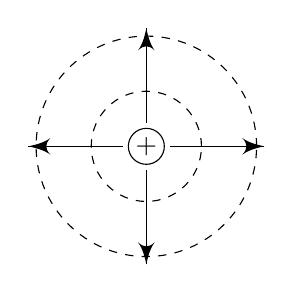
\begin{tikzpicture}
      \node [draw, circle, inner sep = 0, minimum size=13] {+};
      \draw [dashed] circle [radius=1.4];
      \draw [dashed] circle [radius=.7];
      \draw [->] (0, 0.3) -- (0, 1.5);
      \draw [->] (0.3, 0) -- (1.5, 0);
      \draw [->] (0, -0.3) -- (0, -1.5);
      \draw [->] (-0.3, 0) -- (-1.5, 0);
    \end{tikzpicture}
    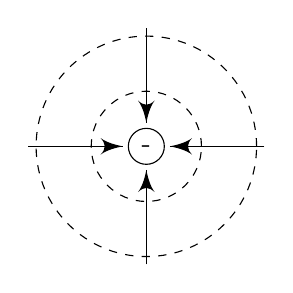
\begin{tikzpicture}
      \node [draw, circle, inner sep = 0, minimum size=13] {-};
      \draw [dashed] circle [radius=1.4];
      \draw [dashed] circle [radius=.7];
      \draw [->] (0, 1.5) -- (0, 0.3);
      \draw [->] (1.5, 0) -- (0.3, 0);
      \draw [->] (0, -1.5) -- (0, -0.3);
      \draw [->] (-1.5, 0) -- (-0.3, 0);
    \end{tikzpicture}
  \end{center}
  Use your imagination to join the two diagrams together to get the field lines for dipoles.
\end{eg}

\subsection{Electrostatic energy}
We want to calculate how much energy is stored in the electric field. Recall from Dynamics and Relativity that a particle of charge $q$ in a field $\mathbf{E} = -\nabla \phi$ has potential energy $U(\mathbf{r}) = q\phi(\mathbf{r})$.

$U(\mathbf{r})$ can be thought of as the work done in bringing the particle from infinity, as illustrated below:
\begin{align*}
  \text{work done} &= -\int_\infty^\mathbf{r} \mathbf{F}\cdot \d \mathbf{r}\\
  &= -\int_\infty^\mathbf{r}\mathbf{E}\cdot \d \mathbf{r} \\
  &= q\int_\infty^\mathbf{r} \nabla \mathbf{\phi}\cdot \d \mathbf{r}\\
  &= q[\phi(\mathbf{r}) - \phi(\infty)]\\
  &= U(\mathbf{r})
\end{align*}
where we set $\phi(\infty) = 0$.

Now consider $N$ charges $q_i$ at positions $\mathbf{r}_i$. The total potential energy stored is the work done to assemble these particles. Let's put them in one by one.
\begin{enumerate}
  \item The first charge is free. The work done is $W_1 = 0$.
  \item To place the second charge at position $\mathbf{r}_2$ takes work. The work is
    \[
      W_2 = \frac{q_1q_1}{4\pi\varepsilon_0}\frac{1}{|\mathbf{r}_1 - \mathbf{r}_2|}.
    \]
  \item To place the third charge at position $\mathbf{r}_3$, we do
    \[
      W_3 = \frac{q_3}{4\pi\varepsilon_0}\left(\frac{q_1}{|\mathbf{r}_1 - \mathbf{r}_3|} - \frac{q_2}{|\mathbf{r}_2 - \mathbf{r}_3|}\right)
    \]
  \item etc.
\end{enumerate}
The total work done is
\begin{prop}
  \[
    U = \sum_{i = 1}^N W_i = \frac{1}{4\pi\varepsilon_0} \sum_{i < j} \frac{q_iq_j}{|\mathbf{r}_i - \mathbf{r}_j|}.
  \]
  Equivalently, 
  \[
    U = \frac{1}{4\pi\varepsilon_0} \frac{1}{2} \sum_{i \not= j} \frac{q_1q_1}{|\mathbf{r}_i - \mathbf{r}_j|}.
  \]
  Now the potential at point $\mathbf{r}_i$ due to all $q_j$ with $j\not= i$ is
  \[
    \phi(\mathbf{r}_i) = \frac{1}{4\pi\varepsilon_0}\sum_{j\not= i}\frac{q}{|\mathbf{r}_i - \mathbf{r}_j|}.
  \]
  So
  \[
    U = \frac{1}{2}\sum_{i = 1}^N q_i \phi(\mathbf{r}_i).
  \]
\end{prop}
There is an obvious generalization to continuous charge distributions:
\begin{prop}
  \[
    U = \frac{1}{2} \int \rho (\mathbf{r}) \phi(\mathbf{r}) \;\d V.
  \]
\end{prop}
\note There is a subtlety here, and there is an extra contribution to the work done in this integral. cf. official notes.

Now we can write
\begin{prop}
  \begin{align*}
    U &= \frac{\varepsilon_0}{2}\int (\nabla\cdot \mathbf{E}) \phi \;\d V\\
    &= \frac{\varepsilon_0}{2}\int [\nabla\cdot (\mathbf{E}\phi) - \mathbf{E}\cdot \nabla \phi]\;\d V\\
    &= \frac{\varepsilon_0}{2}\int \mathbf{E}\cdot \mathbf{E} \;\d V.
  \end{align*}
\end{prop}

\subsection{Conductors}
\begin{defi}[Conductor]
  A \emph{conductor} is a region of space which contains lots of charges that are free to move.
\end{defi}
\note
\begin{itemize}
  \item In electrostatic situations, we must have $\mathbf{E} = 0$ inside a conductor. Otherwise, the charges inside the conductor would move till equilibrium. This almost describes the whole of the section: if you apply an electric field onto a conductor, the charges inside the conductor move until the external field is canceled out.
  \item Since $\mathbf{E} = 0$, $\phi$ is constant inside the conductor.
  \item Since $\nabla \cdot \mathbf{E} = \varepsilon/\varepsilon_0$, $\rho = 0$ inside a conductor, ie. the charges must cancel out inside. So any net charge has to live on the surface.
  \item $\mathbf{E} = -\nabla \phi$ is true, and $\phi$ constant in conductor means $\mathbf{E}$ is perpendicular to the surface.
  \item If there is some surface charge $\sigma$, then the discontinuity of $\mathbf{E}$ gives us $\mathbf{E}_\text{outside} = \frac{\sigma}{\varepsilon_0} \hat{\mathbf{n}}$.
\end{itemize}

There are two typical kinds of problems.
\begin{enumerate}
  \item The total charge $Q$ on a conductor is fixed. 
    \begin{eg}
      Consider a spherical conductor with $Q = 0$ in a constant electric field $\mathbf{E}$. Since the electric field lines must be perpendicular to the surface, they have to bend towards the conductor. Since field lines end and start at charges, there must be negative charges at the left and positive charges at the right.
      \begin{center}
        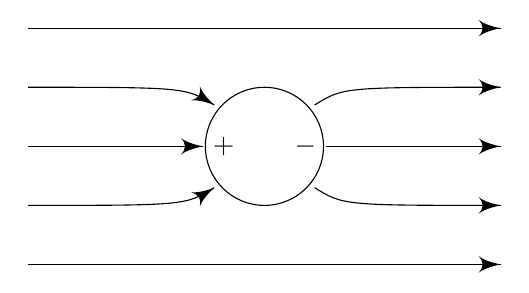
\begin{tikzpicture}
          \draw circle [radius=.75];
          \draw [->] (-3, 1.5) -- (3, 1.5);
          \draw [->] (-3, -1.5) -- (3, -1.5);
          \draw [->] (-3, 0.75) .. controls (-1, 0.75) .. (-.6375, .525);
          \draw [->] (.6375, .525) .. controls (1, 0.75) .. (3, 0.75);
          \draw [->] (-3, -0.75) .. controls (-1, -0.75) .. (-.6375, -.525);
          \draw [->] (.6375, -.525) .. controls (1, -0.75) .. (3, -0.75);
          \draw [->] (-3, 0) -- (-.78, 0) node [right] {$+$};
          \draw [->] (.78, 0) node [left] {$-$} -- (3, 0);
        \end{tikzpicture}
      \end{center}
      We get an induced surface charge and we want to figure out both $\mathbf{E}$ and $\sigma$.
    \end{eg}
  \item The conductor is of fixed potential $\phi$, usually taken to be $\phi = 0$. The conductor is said to be \emph{grounded}, i.e. attached to the Earth.

    \note In the first case, the potential is constant in any particular environment, but can change when the environment changes. In this case, the potential is always 0 regardless of what the world looks like.

    \begin{eg}\leavevmode
      \begin{center}
        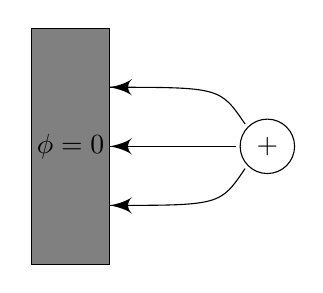
\begin{tikzpicture}
          \draw [fill=gray] (-1, 1.5) rectangle (0, -1.5);
          \node at (-0.5, 0) {$\phi = 0$};
          \node [draw, circle] at (2, 0) {$+$};
          \draw [->] (1.6, 0) -- (0, 0);
          \draw [->] (1.7172, .2828) .. controls (1.4, 0.75) .. (0, 0.75);
          \draw [->] (1.7172, -.2828) .. controls (1.4, -0.75) .. (0, -0.75);
        \end{tikzpicture}
      \end{center}

      Suppose we have a conductor that fills all space $x < 0$. We ground it so that $\phi = 0$ through the plane. Then we place a charge $q$ at $x = d > 0$.

      We are looking for a solution with a source at $x = d$ and $\phi = 0$ at $x = 0$. We know that there is a unique solution.

      We use the method of images, and pretend that instead of a conductor, we have a charge $-q$ at $x = -d$. The potential for this pair is just
      \[
        \phi = \frac{1}{4\pi\varepsilon_0}\left[\frac{q}{\sqrt{(x - d)^2 + y^2 + z^2}} - \frac{q}{\sqrt{(x + d)^2 + y^2 + z^2}}\right].
      \]
      This has $\phi = 0$ at $x = 0$, with a point source at $x = d$. Since this solves our original equation, it must by THE solution.

      We can compute
      \[
        \mathbf{E}_x = -\frac{\partial \phi}{\partial x} = \frac{q}{4\pi\varepsilon_0}\left(\frac{x - d}{|\mathbf{r} - \mathbf{d}|^{3/2}} - \frac{x + d}{|\mathbf{r} + \mathbf{d}|^{3/2}}\right)
      \]
      for $x > 0$. The induced surface charge is
      \[
        \sigma = E_x\varepsilon_0|_{x = 0^+} = -\frac{q}{2\pi}\frac{d}{(d^2 + y^2 + z^2)^{3/2}}.
      \]
      The surface charge is 
      \[
        q = \int \sigma \;\d y\;\d z  = -q.
      \]
    \end{eg}
\end{enumerate}
\section{Magnetostatics}
Charges always give rise to electric fields. Currents give rise to magnetic fields. We will look for time independent solutions to the Maxwell's equation with $\mathbf{J}\not= 0$ and $\rho = 0$. We need to solve
\begin{align*}
  \nabla \times \mathbf{B} &= \mu \mathbf{J}\\
  \nabla\cdot \mathbf{B} &= 0
\end{align*}
The goal is, given $\mathbf{J}$, find $\mathbf{B}$.

\note $\rho = 0$ and $\mathbf{J} \not= 0$ means that we have equal positive and negative charges that can move.

Recall the conservation of charge:
\[
  \frac{\partial\rho}{\partial t} + \nabla \cdot \mathbf{J} = 0.
\]
In this case, since $\rho = 0$, we must have
\[
  \nabla\cdot \mathbf{J} = 0.
\]
These are \emph{steady currents}.
\subsection{Ampere's Law}
Consider a surface $S$ with boundary $C$. Current $\mathbf{J}$ flows through $S$. We now integrate the first equation over the surface $S$ to obtain
\[
  \int_S (\nabla\times \mathbf{B})\cdot \d S = \oint_C \mathbf{B}\cdot \d \mathbf{r} = \mu_0 \int_S \mathbf{J}\cdot \d S.
\]
So
\begin{law}[Ampere's law]
  \[
    \oint_C \mathbf{B}\cdot \d \mathbf{r} = \mu I,
  \]
  where $I$ is the current through the surface.
\end{law}

\begin{eg}[A long straight wire]
  A wire is a cylinder with current $I$ flowing through it.

  We use cylindrical polar coordinates $(r, \varphi, z)$, where $z$ is along the direction of the current, and $r$ points in the radial direction.

  \begin{center}
    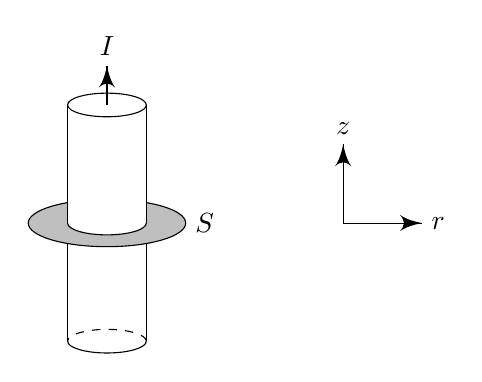
\begin{tikzpicture}
      \draw (0, 1.5) circle [x radius=0.5, y radius = 0.15];
      \draw [dashed] (0.5, -1.5) arc (0: 180:0.5 and 0.15);
      \draw (-0.5, -1.5) arc (180: 360:0.5 and 0.15);
      \draw (0.5, 1.5) -- (0.5, -1.5);
      \draw (-0.5, 1.5) -- (-0.5, -1.5);

      \draw [->] (0, 1.5) -- (0, 2) node [above] {$I$};

      \draw [fill = gray!50!white] circle [x radius = 1, y radius = 0.3];
      \draw [fill = white] circle [x radius = 0.5, y radius = 0.15];
      \draw [fill = white, draw = none] (-0.5, 0) rectangle (0.5, 1);
      \draw (-0.5, 0) -- (-0.5, 1);
      \draw (0.5, 0) -- (0.5, 1);
      \node at (1, 0) [right] {$S$};

      \draw [->] (3, 0) -- (3, 1) node [above] {$z$};
      \draw [->] (3, 0) -- (4, 0) node [right] {$r$};
    \end{tikzpicture}
  \end{center}

  We integrate over a disc that cuts through the wire horizontally.

  We need $\oint_C \mathbf{B}\cdot d\mathbf{r} = \mu_o I$. By symmetry, we have
  \[
    \mathbf{B}(\mathbf{r}) = B(r)\hat{\varphi}.
  \]
  This automatically satisfies $\nabla \cdot \mathbf{B} = 0$.
  Then
  \[
    \oint_C \mathbf{B}\cdot \d \mathbf{r}  =B(r)\int_0^{2\pi} r\;\d \varphi = 2\pi rB(r) = \mu_0 I.
  \]
  So
  \[
    \mathbf{B}(r) = \frac{\mu_0 I}{2\pi r} \hat{\varphi}.
  \]
\end{eg}

\begin{eg}[Surface current]
  Consider the plane $z = 0$ with \emph{surface current density} $\mathbf{k}$ (i.e. current per unit length).
  \begin{center}
     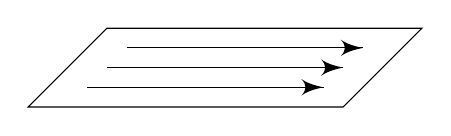
\begin{tikzpicture}[
        y  = {(0.5cm,0.5cm)},
        z  = {(0cm,1cm)}]
      \draw (-2, -1, 0) -- (2, -1, 0) -- (2, 1, 0) -- (-2, 1, 0) -- cycle;
      \draw [->] (-1.5, 0.5, 0) -- (1.5, 0.5, 0);
      \draw [->] (-1.5, -0.5, 0) -- (1.5, -0.5, 0);
      \draw [->] (-1.5, 0, 0) -- (1.5, 0, 0);
    \end{tikzpicture}
  \end{center}

  Take the x-direction to be the direction of the current, and the $z$ direction to be the normal to the plane.

  We imagine this situation by considering to be infinitely many copies of the above wire situation. Then the magnetic fields must point in the $y$-direction. By symmetry, we must have
  \[
    \mathbf{B} = -B(z) \hat{\mathbf{y}},
  \]
  with $B(z) = -B(-z)$.

  Consider a vertical rectangular loop of length $L$ through the surface
  \begin{center}
    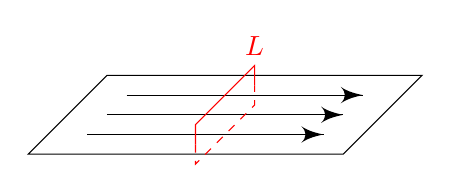
\begin{tikzpicture}[
        y  = {(0.5cm,0.5cm)},
        z  = {(0cm,1cm)}]
      \draw (-2, -1, 0) -- (2, -1, 0) -- (2, 1, 0) -- (-2, 1, 0) -- cycle;
      \draw [->] (-1.5, 0.5, 0) -- (1.5, 0.5, 0);
      \draw [->] (-1.5, -0.5, 0) -- (1.5, -0.5, 0);
      \draw [->] (-1.5, 0, 0) -- (1.5, 0, 0);
      \draw [red] (0, 0.75, 0) -- (0, 0.75, 0.25) node [above] {$L$} -- (0, -0.75, 0.25) -- (0, -0.75, 0);
      \draw [dashed, red] (0, -0.75, 0) -- (0, -0.75, -0.25) -- (0, 0.75, -0.25) -- (0, 0.75, 0);
    \end{tikzpicture}
  \end{center}
  Then
  \[
    \oint_C \mathbf{B}\cdot \d \mathbf{r} = LB(z) - LB(-z) = \mu_0 kL
  \]
  So
  \[
    B(z) = \frac{\mu_0 k}{2}\quad\text{ for }z > 0.
  \]
  Similar to the electrostatic case, the magnetic field is constant, and the part parallel to the surface is discontinuous across the plane. This is a general result, ie. across any surface,
  \[
    \hat {\mathbf{n}} \times \mathbf{B}_+ - \hat{\mathbf{n}}\times \mathbf{B}_{-} = \mu_0 \mathbf{k}.
  \]
\end{eg}

\begin{eg}[Solenoid]
  A \emph{solenoid} is a cylindrical surface current, usually made by wrapping a wire around a cylinder.
  \begin{center}
    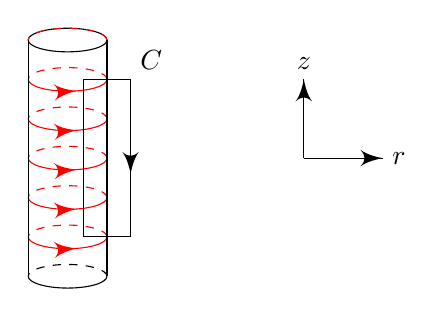
\begin{tikzpicture}
      \draw (0, 1.5) circle [x radius=0.5, y radius = 0.15];
      \draw [dashed] (0.5, -1.5) arc (0: 180:0.5 and 0.15);
      \draw (-0.5, -1.5) arc (180: 360:0.5 and 0.15);
      \draw [red, dashed] (0.5, -1) arc (0: 180:0.5 and 0.15);
      \draw [red, ->-=0.6] (-0.5, -1) arc (180: 360:0.5 and 0.15);
      \draw [red, dashed] (0.5, -0.5) arc (0: 180:0.5 and 0.15);
      \draw [red, ->-=0.6] (-0.5, -0.5) arc (180: 360:0.5 and 0.15);
      \draw [red, dashed] (0.5, 0) arc (0: 180:0.5 and 0.15);
      \draw [red, ->-=0.6] (-0.5, 0) arc (180: 360:0.5 and 0.15);
      \draw [red, dashed] (0.5, 0.5) arc (0: 180:0.5 and 0.15);
      \draw [red, ->-=0.6] (-0.5, 0.5) arc (180: 360:0.5 and 0.15);
      \draw [red, dashed] (0.5, 1) arc (0: 180:0.5 and 0.15);
      \draw [red, ->-=0.6] (-0.5, 1) arc (180: 360:0.5 and 0.15);
      \draw [red, dashed] (0.5, 1.5) arc (0: 180:0.5 and 0.15);
      \draw (0.5, 1.5) -- (0.5, -1.5);
      \draw (-0.5, 1.5) -- (-0.5, -1.5);

      \draw [->] (3, 0) -- (3, 1) node [above] {$z$};
      \draw [->] (3, 0) -- (4, 0) node [right] {$r$};

      \draw (0.2, 1) -- (0.8, 1) node[anchor = south west] {$C$};
      \draw [->-=0.6] (0.8, 1) -- (0.8, -1);
      \draw (0.8, -1) -- (0.2, -1) -- (0.2, 1);
    \end{tikzpicture}
  \end{center}


  We use cylindrical polar coordinates with $z$ in the direction of the extension of the cylinder. By symmetry, $\mathbf{B} = B(r)\mathbf{z}$.

  Away from the cylinder, $\nabla \times \mathbf{B} = 0$. So $\frac{\partial B}{\partial r} = 0$, which means that $B(r)$ is constant outside. Since we know that $\mathbf{B} = \mathbf{0}$ at infinity, $\mathbf{B} = \mathbf{0}$ everywhere outside the cylinder. 

  To compute $\mathbf{B}$ inside, use Ampere's law with a curve $C$. Note that only the vertical part (say of length $L$) inside the cylinder contributes to the integral. Then
  \[
    \oint_C \mathbf{B}\cdot \d \mathbf{r} = BL = \mu_o INL.
  \]
  where $N$ is the number of wires per unit length and $I$ is the current in each wire (so $INL$ is the total amount of current through the wires).

  So $B = \mu_0 IN$.
\end{eg}

\subsection{Vector potential}
For general current distributions $\mathbf{J}$, we also need to solve $\nabla \cdot \mathbf{B} = 0$.

This is telling us that there are no magnetic monopoles, ie. magnetic charges (cf. electric version, with $\rho = 0$)

We can solve this by writing $\mathbf{B} = \nabla \times \mathbf{A}$.
\begin{defi}[Vector potential]
  If $\mathbf{B} = \nabla\times \mathbf{A}$, then $\mathbf{A}$ is the \emph{vector potential}.
\end{defi}
The other Maxwell equation then says
\[
  \nabla \cdot \mathbf{B} = -\nabla^2 \mathbf{A} + \nabla(\nabla\cdot A) = \mu_0 \mathbf{J}.\tag{$*$}
\]

This is rather difficult to solve, but it can be made easier by noting that:
\begin{prop}[Gauge invariance]
  $\mathbf{A}$ is not unique. If $\mathbf{A}$ is a vector potential, then if 
  \[
    \mathbf{A}' = \mathbf{A} + \nabla \chi
  \]
  for any $\chi(\mathbf{x})$, then $\mathbf{B} = \nabla \times \mathbf{A} = \nabla\times \mathbf{A}'$.

  The transformation $\mathbf{A}' \mapsto \mathbf{A} + \nabla\chi$ is called a\emph{gauge transformation}.
\end{prop}

\begin{defi}[(Coulomb) gauge]
  Each $\mathbf{A}$ is called a \emph{gauge}. An $\mathbf{A}$ such that $\nabla \cdot \mathbf{A} = 0$ is called a \emph{Coulomb gauge}.
\end{defi}
\begin{prop}
  We can always pick $\chi$ such that $\nabla \cdot \mathbf{A}' = 0$.
\end{prop}

\begin{proof}
  Suppose that $\mathbf{B} = \nabla \times \mathbf{A}$ with $\nabla \mathbf{A} = \psi(\mathbf{x})$. Then pick $\mathbf{A}' = \mathbf{A} + \nabla \chi$. Then we have
  \[
    \nabla \cdot \mathbf{A}' = \nabla \mathbf{A} + \nabla^2 \chi = \psi + \nabla^2\chi.
  \]
  Pick $\chi$ such that $\nabla^2\chi = -\psi$. This is the Poisson equation and there is always a solution.
\end{proof}

If $\mathbf{B} = \nabla\times \mathbf{A}$ and $\nabla\cdot \mathbf{A} = 0$, then the Maxwell equation  $(*)$ is
\[
  \nabla^2 \mathbf{A} = -\mu_0 \mathbf{J}.
\]

Or, in Cartesian components,
\[
  \nabla^2 A_i = -\mu_0 J_i.
\]
This is 3 copies of the Poisson equation, which we know how to solve using Green's functions. The solution is
\[
  A_i (\mathbf{r}) = \frac{\mu_0}{4\pi}\int \frac{J_i (\mathbf{r}')}{|\mathbf{r} - \mathbf{r}'|}\;\d V,
\]
or
\[
  \mathbf{A}(\mathbf{r}) = \frac{\mu_0}{4\pi}\int \frac{\mathbf{J}(\mathbf{r'})}{|\mathbf{r} - \mathbf{r}'|}\;\d V,
\]
both integrating over $\mathbf{r}'$.

We have to check \emph{Coulomb gauge}:
\begin{align*}
  \nabla\cdot \mathbf{A}(\mathbf{r}) &= \frac{\mu_0}{4\pi}\int \mathbf{J}(\mathbf{r}')\cdot \nabla\left(\frac{1}{|\mathbf{r} - \mathbf{r}'|}\right)\;\d V\\
  &= -\frac{\mu_0}{4\pi}\int \mathbf{J}(\mathbf{r}') \cdot \nabla'\left(\frac{1}{|\mathbf{r} - \mathbf{r}'|}\right)\;\d V\\
  \intertext{We integrate by parts to obtain}
  &= -\frac{\mu_0}{4\pi}\int \left[\nabla'\cdot \left(\frac{\mathbf{J}(\mathbf{r}')}{|\mathbf{r} - \mathbf{r}'|}\right) - \frac{\nabla' \mathbf{J}(\mathbf{r}')}{|\mathbf{r} - \mathbf{r}'|}\right]\;\d V.
\end{align*}
where $\nabla'$ acts on $\mathbf{r}'$. On the last line, the first term vanishes because we have localized current, while the second vanishes because $\nabla \mathbf{F} = 0$. So $\nabla\cdot \mathbf{A} = 0$.

\begin{law}[Biot-Savart law]
  The magnetic field is
  \[
    \mathbf{B}(\mathbf{r}) = \nabla \times \mathbf{A} = \frac{\mu_0}{4\pi}\int \mathbf{J}(\mathbf{r}')\times \frac{\mathbf{r} - \mathbf{r}'}{|\mathbf{r} - \mathbf{r}'|^3}\;\d V.
  \]
  If the current is localized on a curve, this becomes
  \[
    \mathbf{B} = \frac{\mu_0 I}{4\pi}\oint_C \frac{(\mathbf{r} - \mathbf{r}')}{|\mathbf{r} - \mathbf{r}'|^3}\times \d \mathbf{r}',
  \]
  since $\mathbf{J}(\mathbf{r}')$ is non-zero near the curve.
\end{law}

\subsection{Magnetic dipoles}
We want to ask what $\mathbf{B}$ looks like far from a localized current distribution.

\begin{eg}[Current loop]
  Take a current loop of wire $C$, radius $R$ and current $I$. 
  \begin{center}
    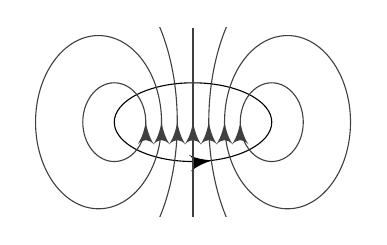
\begin{tikzpicture}
      \clip (-2.1, 1.2) rectangle (2.1, -1.2);
      \draw [->-=0.8] circle [x radius = 1, y radius = 0.5];
      \draw [->, gray!50!black] (-1, 0) circle [x radius=0.4, y radius = 0.5];
      \draw [->, gray!50!black] (-1.2, 0) circle [x radius=0.8, y radius = 1.1];
      \draw [->, gray!50!black] (-1.3, 0) circle [x radius=1.1, y radius = 2];
      \draw [->-=0.5, gray!50!black] (0, -1.2) -- (0, 1.2);
      \draw [gray!50!black] (1, 0) circle [x radius=0.4, y radius = 0.5];
      \draw [gray!50!black] (1.2, 0) circle [x radius=0.8, y radius = 1.1];
      \draw [gray!50!black] (1.3, 0) circle [x radius=1.1, y radius = 2];
      \draw [gray!50!black, ->] (0.6, -0.01) -- (0.6, 0);
      \draw [gray!50!black, ->] (0.4, -0.01) -- (0.4, 0);
      \draw [gray!50!black, ->] (0.2, -0.01) -- (0.2, 0);
    \end{tikzpicture}
  \end{center}
  We can guess that $\mathbf{B}$ looks like this, but we want to calculate it.

  Since $\mathbf{B} = \nabla \times \mathbf{A}$, we know that
  \[
    \mathbf{A}(\mathbf{r}) = \frac{\mu_0}{4\pi}\int\frac{\mathbf{J}(\mathbf{r}')}{|\mathbf{r}-\mathbf{r}'|}\;\d V = \frac{\mu_0 I}{4\pi}\oint_C \frac{\d \mathbf{r}'}{|\mathbf{r} - \mathbf{r}'|}.
  \]
  Far from the loop, $|\mathbf{r} - \mathbf{r}'|$ is small and we can use the Taylor expansion.
  \[
    \frac{1}{|\mathbf{r} - \mathbf{r}'|} = \frac{1}{r} + \frac{\mathbf{r}\cdot \mathbf{r}'}{r^3} + \cdots
  \]
  Then
  \[
    \mathbf{A}(\mathbf{r}) = \frac{\mu_0 I}{r\pi}\oint_C \left(\frac{1}{r} + \frac{\mathbf{r}\cdot \mathbf{r}'}{r^3} + \cdots\right) \d \mathbf{r}'.
  \]
  Note that $r$ is a constant of the integral, and we can take it out. The first $\frac{1}{r}$ term vanishes because it is a constant, and when we integrate along a closed loop, we get 0. So we only consider the second term.

  We claim that for any constant vector $\mathbf{g}$, 
  \[
    \oint_C \mathbf{g}\cdot \mathbf{r}' \;\d \mathbf{r}' = \mathbf{S}\times \mathbf{g},
  \]
  where $\mathbf{S} = \int \d \mathbf{\mathbf{S}}$ is the \emph{vector area} of the surface bounded by $C$. It follows from Green's theorem for the function $f(r')$:
  \[
    \oint f(r')\d \mathbf{r}' = \int_S \nabla f\times\d \mathbf{S},
  \]
  taking $f(r') = \mathbf{g}\cdot \mathbf{r}'$. Then
  \[
    \oint \mathbf{g}\cdot \mathbf{r}'\;\d \mathbf{r}' = \int_S \mathbf{g}\times \d \mathbf{S} = \mathbf{S}\times \mathbf{g}.
  \]
  Using this, we have
  \[
    \mathbf{A}(\mathbf{r}) \approx \frac{\mu_0}{4\pi}\frac{\mathbf{m}\times \mathbf{r}}{r^3},
  \]
  where
  \begin{defi}[Magnetic dipole moment]
    $\mathbf{m} = I\mathbf{S}$ is the \emph{magnetic dipole moment}.
  \end{defi}
  Then
  \[
    \mathbf{B} = \nabla\times \mathbf{A} = \frac{\mu_0}{4\pi}\left(\frac{3(\mathbf{m}\cdot \hat{\mathbf{r}})\hat{\mathbf{r}} - \mathbf{m}}{r^3}\right).
  \]
  This is the same form as $\mathbf{E}$ for an electric dipole, except that there is no $1/r^2$ leading term here, because we have no magnetic monopoles.
\end{eg}

After doing it for a loop, we can do it for a general current distribution:
\begin{eg}
  We have
  \begin{align*}
    A_i(\mathbf{r}) &= \frac{\mu_0}{4\pi}\int \frac{J_i(\mathbf{r}')}{|\mathbf{r} - \mathbf{r}'|}\;\d V\\
    \intertext{Instead of changing it into a line integral, we perform the Taylor expansion directly inside}
    &= \frac{\mu_0}{4\pi}\int\left(\underbrace{\frac{J_i(\mathbf{r}')}{r}}_{\text{vanishes}} - \frac{J_i(\mathbf{r})(\mathbf{r}\cdot \mathbf{r}')}{r^3} + \cdots\right)\;\d V.
  \end{align*}
  To prove that the term actually vanishes, we consider $\partial_j'(J_jr_i')$, where $\partial_i = \frac{\partial}{\partial x_i}$. We have
  \[
    \partial_j'(J_jr_i') = \underbrace{(\partial_j'J_j)}_{=\nabla\cdot \mathbf{J} = 0}r_i' + \underbrace{(\partial_j'r_i')}_{=\delta_{ij}}J_i = J_i.
  \]
  So the 1st term $J_i$ is a total derivative and vanishes as we take the integral over $\R^3$.

  For the second term, we look at
  \[
    \partial_j (J_jr_ir_k) = (\partial_jJ_j)r_ir_k + J_ir_k + J_kr_i =J_kr_i + J_ir_k.
  \]
  Apply this trick to 
  \[
    \int J_ir_jr'_j \;\d V = \int \frac{r_j}{2}(J_i r_j' - J_j r'_i)\;\d V,
  \]
  where we discarded a total derivative $\partial_j'(J_jr_i;r_u')$. Putting it back in vector notation,
  \begin{align*}
    \int J_i\mathbf{r}\cdot \mathbf{r}'\;\d V &= \int\frac{1}{2}\left(J_i(\mathbf{r}\cdot \mathbf{r}') - r_i(\mathbf{J}\cdot \mathbf{r}')\right)\;\d V\\
    &= \int \frac{1}{2}\left[\mathbf{r}\times (\mathbf{J}\times \mathbf{r}')\right]_i\;\d V.
  \end{align*}
  So the long-distance vector potential is again
  \[
    \mathbf{A} (\mathbf{r}) = \frac{\mu_0}{4\pi}\frac{\mathbf{m}\times \mathbf{r}}{r^3},
  \]
  with
  \begin{defi}[Magnetic dipole moment]
    \[
      \mathbf{m} = \frac{1}{2}\int \mathbf{r}'\times \mathbf{J}(\mathbf{r}')\;\d V.
    \]
  \end{defi}
\end{eg}

\subsection{Magnetic forces}
We've seen that moving charge produces currents which generates a magnetic field. But we also know that a charge moving in a magnetic field experiences a force $\mathbf{F} = q\mathbf{r}\times \mathbf{B}$. So the currents will exert a force on each other.

\begin{eg}[Two parallel wires]\leavevmode
  \begin{center}
    \begin{tikzpicture}
      \draw [->-=0.5] (-1, -2) -- (-1, 2);
      \draw [->-=0.5] (1, -2) -- (1, 2);
      \draw [->] (-1, -1.5) -- (1, -1.5) node [pos = 0.5, below] {$d$};
      \draw [->] (1, -1.5) -- (-1, -1.5);

      \draw [->] (3, 0) -- (3, 1) node [above] {$z$};
      \draw [->] (3, 0) -- (4, 0) node [right] {$x$};
      \draw [->] (3, 0) -- (3.8, 0.6) node [anchor = south west] {$y$};
    \end{tikzpicture}
  \end{center}
  We know that the force produced by each current is
  \[
    \mathbf{B}_1 = \frac{\mu_0 I}{2\pi r}\hat{\varphi}.
  \]
  The particles on the second wire will feel as force
  \[
    \mathbf{F} = q\mathbf{r}\times \mathbf{B}_1 = q\mathbf{r}\times \left(\frac{\mu_0 I_1}{2\pi d}\right) \hat{\mathbf{y}}.
  \]
  But $\mathbf{J}_2 = nq\mathbf{v}$ and $I_2 = J_2 A$, where $n$ is the density of particles and $A$ is the cross-sectional area of the wire. So the number of particles per unit length is $nA$, and the force per unit length is
  \[
    \mathbf{f} = na\mathbf{F} = \frac{\mu_0 I_1I_2}{2\pi d}\hat{\mathbf{z}}\times \hat{\mathbf{y}} = -\mu_0\frac{I_1I_2}{2\pi d}\hat{\mathbf{x}}.
  \]
  So if $I_1I_2 > 0$, ie. the currents are in the same direction, the force is attractive. Otherwise the force is repulsive.
\end{eg}

\begin{eg}[General force]
  A current $\mathbf{J}_1$, localized on some closed curve $C_1$, sets up a magnetic field
  \[
    \mathbf{B}(r) = \frac{\mu_0I_1}{4\pi}\oint_{C_1} \frac{\mathbf{r} - \mathbf{r}_1}{|\mathbf{r} - \mathbf{r}_1|^3}\;\d V,
  \]
  integrating over $\mathbf{r}_1$.

  A second current $\mathbf{J}_2$ on $C_2$ experiences the Lorentz force
  \[
    \mathbf{F} = \int \mathbf{J}_2(\mathbf{r})\times \mathbf{B}(\mathbf{r})\;\d V.
  \]
  While we are integrating over all of space, the current is localized at a curve $C-2$. So
  \[
    \mathbf{F} = I_2\oint_{C_2} \d \mathbf{r}_2 \times \mathbf{B}(\mathbf{r}_2).
  \]
  Hence
  \[
    \mathbf{F} = \frac{I_1 I_2}{4\pi}\oint_{C_1}\oint_{C_2}\d \mathbf{r}_2\times \left(\d \mathbf{r}_1\times \frac{\mathbf{r}_2 - \mathbf{r}_1}{|\mathbf{r}_2 - \mathbf{r}_1|^3}\right).
  \]
  For well-separated currents, approximated by $\mathbf{m}_1$ and $\mathbf{m}_2$, we claim that the force can be written as
  \[
    \mathbf{F} = \frac{\mu_0}{4\pi}\nabla\left(\frac{3(\mathbf{m}_1\cdot \hat{\mathbf{r}})(\mathbf{m}_2\cdot \hat{\mathbf{r}}) - (\mathbf{m}_1\cdot \mathbf{m}_2)}{r^3}\right),
  \]
  whose proof is too complicated to be included.
\end{eg}
\note A ``magnet'' we find on fridges consists of many aligned microscopic dipoles

\section{Electrodynamics}
We'll now look at time-dependent $\mathbf{E}$ and $\mathbf{B}$ fields. 
\subsection{Induction}
We'll explore the Maxwell equation
\[
  \nabla\times \mathbf{E} + \frac{\partial \mathbf{B}}{\partial t} = 0.
\]
In short, $\frac{\partial \mathbf{B}}{\partial t} \not = 0$ creates an $\mathbf{E}$ that accelerates charges, which creates a current in a wire. This process is called induction. Consider a wire, which is a closed curve $C$, with a surface $S$.

We integrate over the surface $S$ to obtain
\[
  \int_S (\nabla\times \mathbf{E})\cdot \d \mathbf{S} = \int_S \frac{\partial \mathbf{B}}{\partial t}\cdot \d \mathbf{S}.
\]
By Stokes and commutativity of integration and differentiation (assuming $S$ and $C$ do not change in time), we have
\[
  \int_C \mathbf{E}\cdot \d \mathbf{r} = - \frac{\d }{\d t} \int _S \mathbf{B} \cdot \d \mathbf{S}.
\]
\begin{defi}[Electromotive force (emf)]
  The \emph{electromotive force} (emf) is
  \[
    \mathcal{E} = \int_C \mathbf{E}\cdot \d \mathbf{r}.
  \]
  Note that this is not a force! It's the work done 
\end{defi}

\begin{defi}[Magnetic flux]
  The \emph{magnetic flux} is
  \[
    \Phi = \int_S \mathbf{B}\cdot \d \mathbf{S}.
  \]
\end{defi}
Then we have
\begin{law}[Faraday's law of induction]
  \[
    \mathcal{E} = -\frac{\d \Phi}{\d t}.
  \]
  The minus sign is so important that it has its own name, called \emph{Lenz's law}.
\end{law}

\begin{eg}
  Consider a circular wire with a magnetic file perpendicular to it.
  \begin{center}
    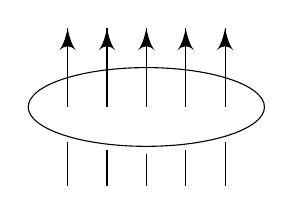
\begin{tikzpicture}
      \draw circle [x radius = 1.5, y radius = 0.5];
      \draw [->] (0, 0) -- (0, 1);
      \draw [->] (-0.5, 0) -- (-0.5, 1);
      \draw [->] (-1, 0) -- (-1, 1);
      \draw [->] (0.5, 0) -- (0.5, 1);
      \draw [->] (1, 0) -- (1, 1);
      \draw (0, -0.6) -- (0, -1); 
      \draw (0.5, -0.55) -- (0.5, -1); 
      \draw (1, -0.45) -- (1, -1); 
      \draw (-0.5, -0.55) -- (-0.5, -1); 
      \draw (-1, -0.45) -- (-1, -1); 
    \end{tikzpicture}
  \end{center}
  If we decrease $\mathbf{B}$ such that $\dot{\Phi} < 0$, then $\mathcal{E} > 0$. So the current flows anticlockwise (viewed from above). The current generates its own $\mathbf{B}$. This acts to \emph{increase} $\mathbf{B}$ inside, which counteracts the initial decrease.
  \begin{center}
    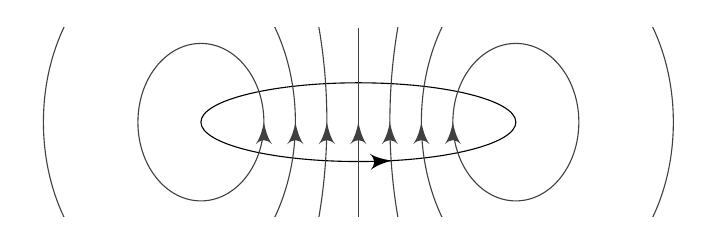
\begin{tikzpicture}[xscale = 2]
      \clip (-2.1, 1.2) rectangle (2.1, -1.2);
      \draw [->-=0.8] circle [x radius = 1, y radius = 0.5];
      \draw [->, gray!50!black] (-1, 0) circle [x radius=0.4, y radius = 1];
      \draw [->, gray!50!black] (-1.2, 0) circle [x radius=0.8, y radius = 2.2];
      \draw [->, gray!50!black] (-1.3, 0) circle [x radius=1.1, y radius = 4];
      \draw [->-=0.5, gray!50!black] (0, -1.2) -- (0, 1.2);
      \draw [gray!50!black] (1, 0) circle [x radius=0.4, y radius = 1];
      \draw [gray!50!black] (1.2, 0) circle [x radius=0.8, y radius = 2.2];
      \draw [gray!50!black] (1.3, 0) circle [x radius=1.1, y radius = 4];
      \draw [gray!50!black, ->] (0.6, -0.01) -- (0.6, 0);
      \draw [gray!50!black, ->] (0.4, -0.01) -- (0.4, 0);
      \draw [gray!50!black, ->] (0.2, -0.01) -- (0.2, 0);
    \end{tikzpicture}
  \end{center}
  This means you don't get runaway behaviour.
\end{eg}
There is a related way to induce a current: keep $\mathbf{B}$ fixed and move wire.

\begin{eg}\leavevmode
  \begin{center}
    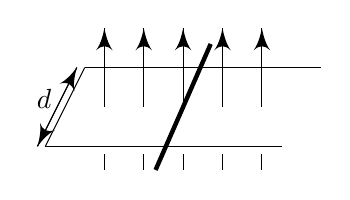
\begin{tikzpicture}
      \draw (0, 0) -- (3, 0);
      \draw (0, 0) -- (0.5, 1);
      \draw [->] (0.4, 1) -- (-0.1, 0) node [pos = 0.4, left] {$d$};
      \draw [->] (-0.1, 0) -- (0.4, 1);
      \draw (0.5, 1) -- (3.5, 1);
      \draw [ultra thick] (1.4, -0.3) -- (2.1, 1.3);
      \draw (0.75, -0.1) -- (0.75, -0.3);
      \draw (1.25, -0.1) -- (1.25, -0.3);
      \draw (1.75, -0.1) -- (1.75, -0.3);
      \draw (2.25, -0.1) -- (2.25, -0.3);
      \draw (2.75, -0.1) -- (2.75, -0.3);
      \draw [->] (0.75, 0.5) -- (0.75, 1.5);
      \draw [->] (1.25, 0.5) -- (1.25, 1.5);
      \draw [->] (1.75, 0.5) -- (1.75, 1.5);
      \draw [->] (2.25, 0.5) -- (2.25, 1.5);
      \draw [->] (2.75, 0.5) -- (2.75, 1.5);
    \end{tikzpicture}
  \end{center}

  Slide bar to the left with speed $v$. Each charge $q$ will experience a Lorentz force
  \[
    F = qvB,
  \]
  in the counterclockwise direction.

  The emf, defined as the work done per unit charge, is
  \[
    \mathcal{E} = vBd,
  \]
  because work is only done for particles on the bar.

  Meanwhile, the change of flux is
  \[
    \frac{\d \Phi}{\d t} = -vBd,
  \]
  since the area decreases at a rate of $-vd$.

  We again have
  \[
    \mathcal{E} = -\frac{\d \Phi}{\d t}.
  \]
  Note that we obtain the same formula but different physics - we used Lorentz force law, not Maxwell's equation.
\end{eg}

Now we consider the general case: a moving loop $C(t)$ bounding a surface $S(t)$.  As the curve moves, the curve sweeps out a cylinder $S_c$.

The change in flux
\begin{align*}
  \Phi(t + \delta t) - \Phi(t) &= \int_{S(t + \delta t)} \mathbf{B}(t + \delta t)\cdot \d \mathbf{S} - \int_{S(t)}\mathbf{B}(t)\cdot \d \mathbf{S}\\
  &= \int_{S(t + \delta t)}\left(\mathbf{B}(t) + \frac{\partial \mathbf{B}}{\partial t}\right)\cdot \d \mathbf{S} - \int_{S(t)}\mathbf{B}(t)\cdot \d \mathbf{S} + O(\delta t^2)\\
  &= \int_{S(t)}\frac{\partial \mathbf{B}}{\partial t}\cdot \d \mathbf{S} + \left[\int_{S(t + \delta t)} - \int_{S(t)}\right]\mathbf{B}(t)\cdot \d \mathbf{S} + O(\delta t^2)
\end{align*}
We know that
\[
  \left[\int_{S(t + \delta t)} - \int_{S(t)}\right]\mathbf{B}(t)\cdot \d \mathbf{S} + \int_{S_c}\mathbf{B}(t)\cdot \d \mathbf{S} = 0,
\]
since the integral of $\mathbf{B}$ over a closed surface is 0.

Write surface element on $S_c$ as
\[
  \d \mathbf{S} = (\d \mathbf{r}\times \mathbf{v})\;\d t.
\]
Then
\[
  \frac{\d \Phi}{\d t} = \lim_{\delta \to 0}\frac{\delta \Phi}{\delta t} = \int_{S(t)}\frac{\partial \mathbf{B}}{\partial t}\cdot \d \mathbf{S} - \int_{c(t)}(\mathbf{v}\times \mathbf{B}\cdot \d \mathbf{r}.
\]
Using Maxwell's equation, we have
\[
  \frac{\d \Phi}{\d t} = -\int_C (\mathbf{E} + \mathbf{v}\times \mathbf{B})\;\d \mathbf{r}.
\]
which is the emf $\mathcal{E}$ in general.
\subsection{Magnetostatic energy}
Suppose that a current $I$ flows along a wire $C$. From magnetostatics, we know that this gives rise to a magnetic field $\mathbf{B}$, and hence a flux $\Phi$ given by
\[
  \Phi = \int_S \mathbf{B}\cdot \d \mathbf{S},
\]
where $S$ is the surface bounded by $C$.
\begin{defi}[Inductance]
  The \emph{inductance} of a $C$
  \[
    L = \frac{\Phi}{I},
  \]
  the amount of flux it generates per unit current passing through $C$. It is a property only of the curve $C$.
\end{defi}
While this concept is very important in engineering, the only place it will appear in this course is in the coming proof.

\begin{eg}[The solenoid]
  Consider a solenoid of length $\ell$ and cross-sectional area $A$ (with $\ell \gg \sqrt{A}$ so we can ignore end effects). We know that
  \[
    B = \mu_0 IN,
  \]
  where $N$ is the number of turns of wire per unit length and $I$ is the current. The flux through a single turn (pretending it is closed) is
  \[
    \Phi_0 = \mu_0 INA.
  \]
  So the total flux is
  \[
    \Phi = \Phi_0 N\ell = \mu_0 IN^2V,
  \]
  where $V$ is the volume, $A\ell$. So
  \[
    L = \mu_0 N^2 V.
  \]
\end{eg}

We can use the idea of inductance to compute the energy stored in magnetic fields. The idea is to compute the work done in building up a current.

Take a current $I$. Changing the current $\Rightarrow$ magnetic field chances $\Rightarrow$ induced emf,
\[
  \mathcal{E} = -\frac{\d \Phi}{\d t} = -L\frac{\d I}{\d t}.
\]
This opposes the change in current by Lenz's law. In time $\delta t$, a charge $I\delta t$ flows around $C$. The work done is
\[
  \delta W = \mathcal{E} I\delta t = -LI\frac{\d I}{\d t}\delta t.
\]
So
\[
  \frac{\d W}{\d t} = -LI \frac{\d I}{\d t} = -\frac{1}{2}L\frac{\d I^2}{\d t}.
\]
So the work done to build up a current is
\[
  W = \frac{1}{2}LI^2 = \frac{1}{2}I\Phi.
\]
Note that we dropped the minus sign because we switched from talking about the work done by the emf to the work done to oppose the emf.

This is identified with the energy stored in the system,
\begin{align*}
  U &= \frac{1}{2}I\int_S \mathbf{B}\cdot \d \mathbf{S}\\
  &= \frac{1}{2}I\int_S(\nabla\times \mathbf{A})\cdot \d \mathbf{S}\\
  &= \frac{1}{2}I\oint_C \mathbf{A}\cdot \d \mathbf{r}\quad\text{using Stokes'}\\
  &= \frac{1}{2}\int_{\R^3} \mathbf{J}\cdot \mathbf{A}\;\d V\\
  \intertext{Using Maxwell's equation $\nabla\times \mathbf{B} = \mu_0 \mathbf{J}$,}
  &= \frac{1}{2\mu_0}\int (\nabla\times \mathbf{B})\cdot \mathbf{A}\;\d V\\
  &= \frac{1}{2\mu_0}\int[\underbrace{\nabla\cdot(\mathbf{B}\times \mathbf{A})}_{\text{vanishes if }C\text{ is localized}} + \mathbf{B}\cdot (\nabla\times \mathbf{A})]\;\d V\\
  &= \frac{1}{2\mu_0}\int \mathbf{B}\cdot \mathbf{B}\;\d V.
\end{align*}
So
\begin{prop}
  The energy stored in a magnetic field is
  \[
    U = \frac{1}{2\mu_0}\int \mathbf{B}\cdot \mathbf{B}\;\d V.
  \]
\end{prop}
In general, the energy stored in $\mathbf{E}$ and $\mathbf{B}$ is
\[
  U = \int \left(\frac{\varepsilon_0}{2}\mathbf{E}\cdot \mathbf{E} + \frac{1}{2\mu_0}\mathbf{B}\cdot \mathbf{B}\right)\;\d V.
\]
Note that this does not follow from our results for pure magnetic fields and pure electric fields, since when both are present, they might interact in weird ways.

\subsection{Resistance}
The story so far is 
\[
  \frac{\d \Phi}{\d t} = -\mathcal{E} \Rightarrow \text{\emph{accelerates} charges}
\]
In principle, we should be able to compute the current. But accelerating charges are complicated (emit light). Instead, we invoke a new effect, friction.

In a wire, this is called \emph{resistance}. In most materials, the effect of resistance is that $\mathcal{E}$ is proportional to the speed of the charged particles, rather than the acceleration.

We can think of the particles as accelerating for a very short period of time, and then reaching a terminal velocity. So
\begin{law}[Ohm's law]
  \[
    \mathcal{E} = IR,
  \]
\end{law}
\begin{defi}[Resistance]
  The \emph{resistance} is the $R$ in Ohm's law.
\end{defi}
\note $\mathcal{E} = \int \mathbf{E}\;\d \mathbf{r}$ and $\mathbf{E} = - \nabla\phi$. So $\mathcal{E} = V$, the potential difference. So Ohm's law says $V = IR$.

\begin{defi}{Resistivity and conductivity}
For the wire of length $L$ and cross-sectional area $A$, we define the \emph{resistivity} to be
\[
  \rho = \frac{AR}{L},
\]
and the conductivity is
\[
  \sigma = \frac{1}{\rho}.
\]
\end{defi}
These are properties only of the substance and not the actual shape of the wire. Then Ohm's law reads
\begin{law}[Ohm's law]
  \[
    \mathbf{J} = \sigma \mathbf{E}.
  \]
\end{law}
We can formally derive Ohm's law by considering the field and interactions between the electron and the atoms, but we're not going to do that.

\begin{eg}\leavevmode
  \begin{center}
    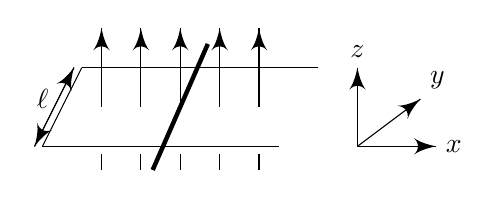
\begin{tikzpicture}
      \draw (0, 0) -- (3, 0);
      \draw (0, 0) -- (0.5, 1);
      \draw [->] (0.4, 1) -- (-0.1, 0) node [pos = 0.4, left] {$\ell$};
      \draw [->] (-0.1, 0) -- (0.4, 1);
      \draw (0.5, 1) -- (3.5, 1);
      \draw [ultra thick] (1.4, -0.3) -- (2.1, 1.3);
      \draw (0.75, -0.1) -- (0.75, -0.3);
      \draw (1.25, -0.1) -- (1.25, -0.3);
      \draw (1.75, -0.1) -- (1.75, -0.3);
      \draw (2.25, -0.1) -- (2.25, -0.3);
      \draw (2.75, -0.1) -- (2.75, -0.3);
      \draw [->] (0.75, 0.5) -- (0.75, 1.5);
      \draw [->] (1.25, 0.5) -- (1.25, 1.5);
      \draw [->] (1.75, 0.5) -- (1.75, 1.5);
      \draw [->] (2.25, 0.5) -- (2.25, 1.5);
      \draw [->] (2.75, 0.5) -- (2.75, 1.5);

      \draw [->] (4, 0) -- (4, 1) node [above] {$z$};
      \draw [->] (4, 0) -- (5, 0) node [right] {$x$};
      \draw [->] (4, 0) -- (4.8, 0.6) node [anchor = south west] {$y$};
    \end{tikzpicture}
  \end{center}
  Suppose the bar moves to the left with speed $v$. Suppose that the sliding bar has resistance $R$, and the remaining parts of the circuit are superconductors.

  There are two dynamical variables, the position of the bar $x(t)$, and the current $I(t)$.

  If a current $I$ flows, the force on a small segment of the bar is
  \[
    \mathbf{F} = IB \hat{\mathbf{y}}\times \hat{\mathbf{z}}
  \]
  So the total force on a bar is
  \[
    \mathbf{F} = IB\ell\hat{x}.
  \]
  So
  \[
    m\ddot{\mathbf{x}} = IB\ell.
  \]
  To determine the current
  \[
    \mathcal{E} = -\frac{\d \Phi}{\d t} = -BD\dot{\mathbf{x}}.
  \]
  So Ohm's law gives
  \[
    IR = -B\ell\dot{x}.
  \]
  Hence
  \[
    m\ddot{x} = -\frac{B^2\ell^2}{R}\dot{x}.
  \]
  Integrating once gives
  \[
    \dot{x}(t) = -ve^{-B^2\ell^2t/mR}.
  \]
\end{eg}
With resistance, we need to do work to keep a constant current. In time $\delta t$, the work needed is
\[
  \delta W = \mathcal{E} I\delta t = I^2 R \delta t
\]
using Ohm's law. So
\begin{defi}[Joule heating]
  \emph{Joule heating} is the energy lost in a circuit due to friction. It is given by
  \[
    \frac{\d W}{\d t} = I^2 R.
  \]
\end{defi}
\subsection{Electromagnetic waves}
Recall that the Maxwell equations are
\begin{align*}
  \nabla \cdot \mathbf{E} &= \frac{\rho}{\varepsilon_0}\\
  \nabla \cdot \mathbf{B} &= 0\\
  \nabla \times \mathbf{E} &= -\frac{\partial \mathbf{E}}{\partial t}\\
  \nabla \times \mathbf{B} &= \mu_0\left(\mathbf{J} + \varepsilon_0 \frac{\partial \mathbf{E}}{\partial t}\right)
\end{align*}
So far we have studied all the equations apart from the $\mu_0\varepsilon_0 \frac{\partial \mathbf{E}}{\partial t}$ term. Historically this term is called the \emph{displacement current}.

The need of this term was discovered by purely mathematically, since people discovered that Maxwell's equations would be inconsistent with charge conservation without the term.

Without the term, the last equation is
\[
  \nabla \times \mathbf{B} = \mu_0 \mathbf{J}.
\]
Take the divergence of the equation to obtain
\[
  \mu_0 \nabla\cdot \mathbf{J} = \nabla\cdot (\nabla\times \mathbf{B}) = 0.
\]
But charge conservation says that
\[
  \dot{\rho} + \nabla\cdot \mathbf{J} = 0.
\]
These can both hold iff $\dot{\rho} = 0$. But we clearly can change the charge density - pick up a charge and move it elsewhere! Contradiction.


With the new term, taking the divergence yields
\[
  \mu_0\left(\nabla\cdot \mathbf{J} + \epsilon_0 \nabla\cdot \frac{\partial \mathbf{E}}{\partial t}\right) = 0.
\]
Since partial derivatives commute, we have
\[
  \varepsilon_0\nabla\cdot \frac{\partial \mathbf{E}}{\partial t} = \varepsilon_0 \frac{\partial}{\partial t} (\nabla\cdot \mathbf{E}) = \dot{\rho}
\]
by the first Maxwell's equation. So it gives
\[
  \nabla\cdot \mathbf{J} + \dot{\rho} = 0.
\]
So with the new term, not only is Maxwell's equation consistent with charge conservation - it actually implies charge conservation.

We now look for solutions to Maxwell's equation in the case where $\rho = 0$ and $\mathbf{J} = 0$, ie. in nothing/vacuum.

Differentiating the fourth equation with respect to time,
\begin{align*}
  \mu_0\varepsilon_0 \frac{\partial^2 \mathbf{E}}{\partial t^2} &= \frac{\partial }{\partial t}(\nabla\times \mathbf{B})\\
  &= \nabla\times \frac{\partial B}{\partial t}\\
  &= \nabla(\underbrace{\nabla\cdot \mathbf{E}}_{ = \rho/\varepsilon_0 = 0}) + \nabla^2 \mathbf{E}\quad \text{ by vector identities}\\
  &= \nabla^2 \mathbf{E}.
\end{align*}
So each component of $\mathbf{E}$ obeys the wave equation
\[
  \frac{1}{c^2}\frac{\partial^2 \mathbf{E}}{\partial t^2} - \nabla^2 \mathbf{E} = 0.
\]
We can do exactly the same thing to show that $\mathbf{B}$ obeys the same equation:
\[
  \frac{1}{c^2}\frac{\partial^2 \mathbf{B}}{\partial t^2} - \nabla^2 \mathbf{B} = 0,
\]
where the speed of the wave is
\[
  c = \frac{1}{\sqrt{\mu_0\varepsilon_0}}
\]
Recall from the first lecture that
\begin{itemize}
  \item $\varepsilon_0 = \SI{8.85e-12}{\per\metre\cubed\per\kilogram\s\squared\coulomb\squared}$
  \item $\mu_0 = \SI{4\pi e-6}{\metre\kilogram\per\coulomb\squared}$
\end{itemize}
So
\[
  c = \SI{3e8}{\meter\per\second},
\]
which is the speed of light!

We now look for plane wave solutions which propagate in the $x$ direction, and are independent of $y$ and $z$. So any derivatives wrt $y$ and $z$ are zero (ie doesn't change if we move in the $y$ or $z$ direction). So
\[
  \nabla\cdot \mathbf{E} = 0 \Rightarrow  E_x\text{ is constant}
\]
We take $E_x = 0$. wlog, assume $E_z = 0$, ie the wave propagate in the $x$ direction and oscillates in the $y$ direction. Then we look for solutions of the form
\[
  \mathbf{E} = (0, E(x, t), 0).
\]
With
\[
  \frac{1}{c^2}\frac{\partial^2 \mathbf{E}}{\partial t^2} - \frac{\partial^2 E}{\partial x^2}\mathbf{E} = 0.
\]
The general solution is
\[
  E(x, t) = f(x - ct) + g(x + ct).
\]
The most important solutions are the \emph{monochromatic} waves
\[
  E = E_0 \sin (kx - \omega t).
\]
\begin{defi}[Amplitude, wave number and frequency]\leavevmode
  \begin{enumerate}
    \item $E_0$ is the \emph{amplitude}
    \item $k$ is the \emph{wave number}.
    \item $\omega$ is the \emph{(angular) frequency}.
  \end{enumerate}
  The wave number is related to the wavelength by
  \[
    \lambda = \frac{2\pi}{k}.
  \]
  Since the wave has to travel at speed $c$, we must have
  \[
    \omega^2 = c^2 k^2
  \]
  So the value of $k$ determines the value of $\omega$, vice versa.
\end{defi}
To solve for $\mathbf{B}$,we use
\[
  \nabla\times \mathbf{E} = -\frac{\partial \mathbf{B}}{\partial t}.
\]
So $\mathbf{B} = (0, 0, B)$ for some $B$. Hence the equation gives.
\[
  \frac{\partial B}{\partial t} = -\frac{\partial E}{\partial x}.
\]
So
\[
  B = \frac{E_0}{c}\sin(kx - \omega t).
\]
Note that this is uniquely determined by $\mathbf{E}$, and we do not get to choose our favorite amplitude, frequency etc for the magnetic component.

We see that $\mathbf{E}$ and $\mathbf{B}$ oscillate in phase, orthogonal to each other, and orthogonal to the direction of travel. These waves are what we usually consider to be ``light''.

Also note that Maxwell's equations are linear, so we can add up two solutions to get a new one.

It is useful to sue complex notation. The most general monochromatic takes the form
\[
  \mathbf{E} = \mathbf{E}_0 \exp(i(\mathbf{k}\cdot \mathbf{x} - \omega t)),
\]
and
\[
  \mathbf{B} = \mathbf{B}_0 \exp(i(\mathbf{k}\cdot \mathbf{x} - \omega t)),
\]
with $\omega = c^2 |\mathbf{k}|^2$.
\begin{defi}[Wave vector]
  $\mathbf{k}$ is the \emph{wave vector}, which is real.
\end{defi}
The ``actual'' solutions are just the real part of these expressions.

There are some restrictions to the values of $\mathbf{E}_0$ etc due to the maxwell's equations:

\begin{align*}
  \nabla\cdot \mathbf{E} = 0 &\Rightarrow \mathbf{k}\cdot \mathbf{E}_0 = 0\\
  \nabla\cdot \mathbf{B} = 0 &\Rightarrow \mathbf{k}\cdot \mathbf{B}_0 = 0\\
  \nabla\times \mathbf{E} = -\frac{\partial \mathbf{B}}{\partial t} &\Rightarrow \mathbf{k}\times \mathbf{E}_0 = \omega \mathbf{B}_0
\end{align*}
If $\mathbf{E}_0$ and $\mathbf{B}_0$ are real, then $\mathbf{k}, \mathbf{E}_0/c$ and $\mathbf{B}_0$ form a right-handed orthogonal triad of vectors.
\begin{defi}[Linearly polarized wave]
  A solution with real $\mathbf{E}_0, \mathbf{B}_0, \mathbf{k}$ is said to be \emph{linearly polarized}.
\end{defi}
This says that the waves oscillate up and down in a fixed plane.

If $\mathbf{E}_0$ and $\mathbf{B}_0$ are complex, then the polarization is not in a fixed direction. If we write
\[
  \mathbf{E}_0 = \boldsymbol\alpha + i\boldsymbol\beta
\]
for $\boldsymbol\alpha, \boldsymbol\beta\in \R^3$, then the ``real solution'' is
\[
  \re(\mathbf{E}) = \boldsymbol\alpha\cos(\mathbf{k}\cdot \mathbf{x} - \omega t) - \boldsymbol\beta \sin (\mathbf{k}\cdot \mathbf{x} - \omega t).
\]
Note that $\nabla\cdot \mathbf{E} = 0$ requires that $\mathbf{k}\cdot \boldsymbol\alpha = \mathbf{k}\cdot \boldsymbol\beta$. It is not difficult to see that this traces out an ellipse.
\begin{defi}[Elliptically polarized wave]
  If $\mathbf{E}_0$ and $\mathbf{B}_0$ are complex, then it is said to be \emph{elliptically polarized}. In the special case where $|\boldsymbol\alpha| = |\boldsymbol\beta|$ and $\boldsymbol\alpha \cdot \boldsymbol\beta = 0$, this is \emph{circular polarization}.
\end{defi}

We can have a simple application: why metals are shiny.

A metal is a conductor. Suppose the region $x > 0$ is filled with a conductor.
\begin{center}
  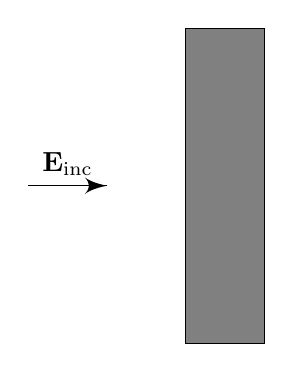
\begin{tikzpicture}
    \draw [fill=gray] (0, 2) rectangle (1, -2);
    \draw [->] (-2, 0) -- (-1, 0) node [pos =0.5, above] {$\mathbf{E}_\mathrm{inc}$};
  \end{tikzpicture}
\end{center}
A light wave is incident on the conductor, ie
\[
  \mathbf{E}_{\mathrm{inc}} = E_0 \hat{\mathbf{y}} \exp(i(kx + \omega t)),
\]
with $\omega = ck$.

We know that inside a conductor, $\mathbf{E} = 0$, and at the surface, $\mathbf{E}_{\parallel} = 0$. So $\mathbf{E}_0 \cdot \hat{\mathbf{y}}|_{x = 0} = 0$.

Then clearly our solution above does not satisfy the boundary conditions!

To achieve the boundary conditions, we add a reflected wave
\[
  \mathbf{E}_{\mathrm{ref}} = -E_0 \hat{\mathbf{y}} \exp(i(-kx - \omega t)).
\]
Then our total electric field is
\[
  \mathbf{E} = \mathbf{E}_{\mathrm{inc}} + \mathbf{E}_{\mathrm{ref}}.
\]
Then this is a solution to Maxwell's equations since it is a sum of two solutions, and satisfies $\mathbf{E}\cdot \hat{\mathbf{y}}|_{x = 0} = 0$ as required.

Maxwell's equations says $\nabla\times \mathbf{E} = -\frac{\partial \mathbf{B}}{\partial t}$. So
\begin{align*}
  \mathbf{B}_{\mathrm{inc}} &= \frac{E_0}{c}\hat{\mathbf{z}} \exp(i(kx - \omega t))\\
  \mathbf{B}_{\mathrm{ref}} &= \frac{E_0}{c}\hat{\mathbf{z}} \exp(i(-kx - \omega t))
\end{align*}
This obeys $\mathbf{B}\cdot \hat{\mathbf{n}} = 0$, where $\hat{\mathbf{n}}$ is the normal to the surface. But we also have
\[
  \mathbf{B}\cdot \hat{\mathbf{z}}|_{x = 0} = \frac{2E_0}{c}e^{-i\omega t},
\]
and $\mathbf{B} = 0$ inside the conductor. So there \emph{is} a magnetic field at the surface.

By our boundary conditions for conductors, this means that there's a surface current! This is given by
\[
  \mathbf{K} = \pm\frac{2E_0}{\mu_0 c}\hat{\mathbf{y}} e^{-i \omega t}.
\]
So shining a light onto a metal will cause an oscillating current. We can imagine the process as the incident light hits the conductor, causes an oscillating current, which generates a reflected wave (since accelerating charges generate light - cf. next year)

We can do the same for light incident at an angle, and prove that the incident angle is equal to the reflected angle.

\subsection{Poynting vector}
Electromagnetic waves carry energy - that's how the Sun heats up the Earth! We will compute how much.

The energy stored in a field in a volume $V$ is
\[
  U = \int_V \left(\frac{\varepsilon_0}{2}\mathbf{E}\cdot \mathbf{E} + \frac{1}{2\mu_0}\mathbf{B}\cdot \mathbf{B}\right)\;\d V.
\]
We have
\begin{align*}
  \frac{\d U}{\d t} &= \int_V \left(\varepsilon_0 \mathbf{E}\cdot \frac{\partial \mathbf{E}}{\partial t} + \frac{1}{\mu_0}\mathbf{B}\cdot \frac{\partial \mathbf{B}}{\partial t}\right)\;\d V\\
  &= \int_V \left(\frac{1}{\mu_0}\mathbf{E}\cdot (\nabla\times \mathbf{B}) - \mathbf{E}\cdot \mathbf{J} - \frac{1}{\mu_0}\mathbf{B}\cdot (\nabla\times \mathbf{E})\right).
\end{align*}
But
\[
  \mathbf{E}\cdot (\nabla \times \mathbf{B}) - \mathbf{B}\cdot (\nabla\times \mathbf{E}) = \nabla\cdot (\mathbf{E}\times \mathbf{B}),
\]
by vector equations. So
\[
  \frac{\d U}{\d t} = -\int_V \mathbf{J}\cdot \mathbf{E}\;\d V - \frac{1}{\mu_0}\int_S (\mathbf{E}\times \mathbf{B}\cdot \;\d \mathbf{S}.
\]
Recall that the work done on a particle $q$ moving with velocity $v$ is $\delta W = q\mathbf{v}\cdot \mathbf{E}\;\delta t$. So the $\mathbf{J}\cdot \mathbf{E}$ term is the work done on a charged particles in $V$. We can thus write
\begin{thm}[Poynting theorem]
  \[
    \underbrace{\frac{\d U}{\d t} + \int_V J\cdot \mathbf{E} \;\d V}_{\text{Total change of energy in $V$ (fields + particles)}} = \underbrace{-\frac{1}{\mu_0}\int_S (\mathbf{E}\times \mathbf{B}\cdot\d S}_{\text{Energy that escapes through the surface }S}.
  \]
\end{thm}

\begin{defi}[Poynting vector]
  The \emph{Poynting vector} is
  \[
    \mathbf{S} = \frac{1}{\mu_0}\mathbf{E}\times \mathbf{B}.
  \]
\end{defi}
This characterizes the energy transfer.

For a linearly polarized wave, 
\begin{align*}
  \mathbf{E} &= \mathbf{E}_0 \sin (\mathbf{k}\cdot \mathbf{x} - \omega t)\\
  \mathbf{B} &= \frac{1}{c}(\hat{\mathbf{k}}\times \mathbf{E}_0)\sin (\mathbf{k}\cdot \mathbf{x} - \omega t).
\end{align*}
So
\[
  \mathbf{S} = \frac{cE_0^2}{\mu_0}\hat{\mathbf{k}} \sin^2(\mathbf{k}\\mathbf{x} - \omega t).
\]
The average over $T = \frac{2\pi}{\omega}$ is thus
\[
  \bra\mathbf{S}\ket = \frac{cE_0^2}{2\mu_0}\hat{\mathbf{k}}.
\]
\end{document}
